\section{Erzeugung von Elementarteilchen}
% --------------------------------------------------
\begin{frame}
  \frametitle{Wie k\"onnen wir neue Teilchen erzeugen?}
  \pause
  \begin{block}{}
    \begin{columns}
     \begin{column}{0.3\textwidth}
        \centering
        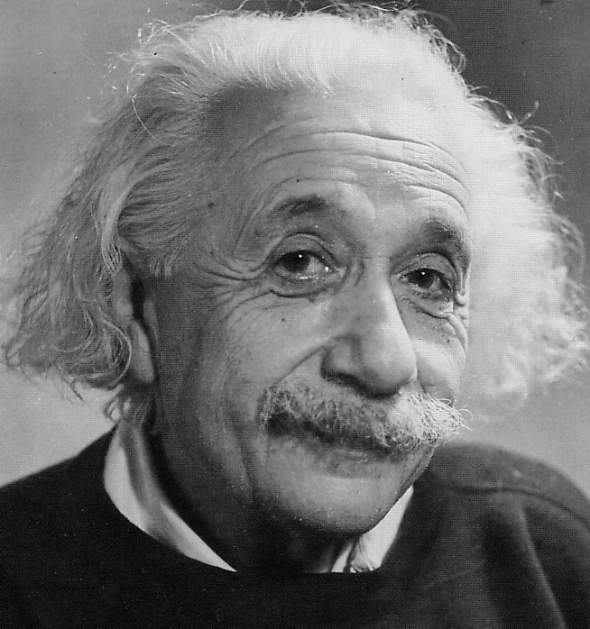
\includegraphics[width=0.5\textwidth]{eyecandy/einstein55}
      \end{column}
      \pause
      \begin{column}{0.7\textwidth}
        \alert{``Masse entspricht Energie''}
        \begin{equation*}
          \hskip-4cm
          E = m\cdot c^{2} \quad\Leftrightarrow\quad m = \frac{E}{c^{2}}
       \end{equation*}
   \end{column}
    \end{columns}
  \end{block}
  \pause
  \begin{itemize}
  \item Kollision von zwei Teilchen mit jeweils Energie $E$
  \end{itemize}
  \centering
  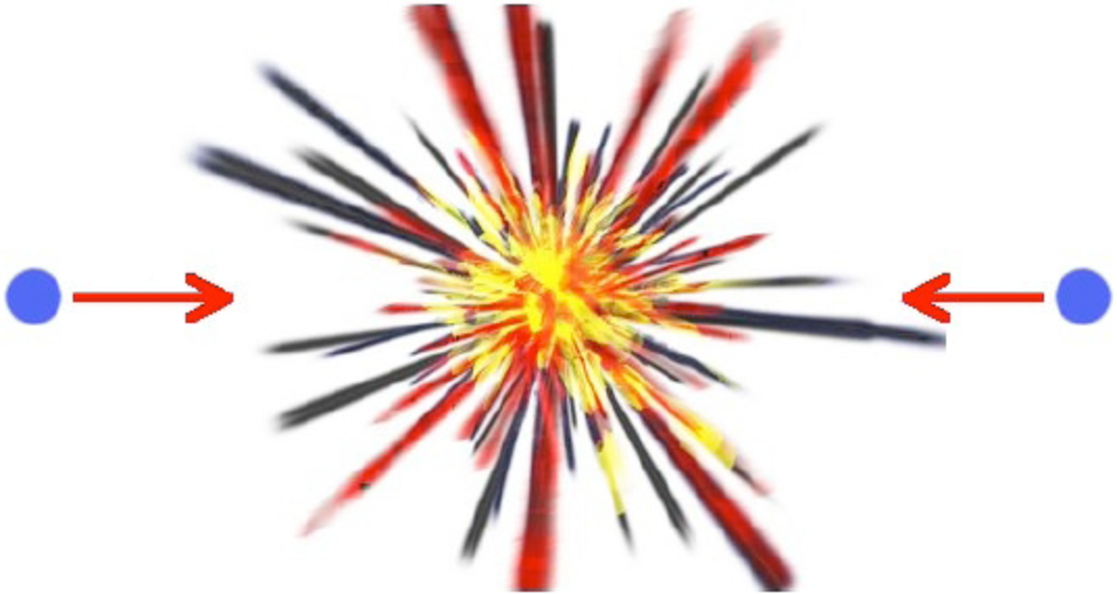
\includegraphics[width=0.55\textwidth]{lhc/Collision}
  \begin{itemize}
  \item[$\Rightarrow$] Erzeugung neuer Teilchen bis zur Masse $2m = 2E
    \quad(c=1)$
  \end{itemize}
\end{frame}

% --------------------------------------------------
\begin{frame}
  \frametitle{Woher bekommt man schnelle Teilchen?}
  \pause
  \begin{center}
    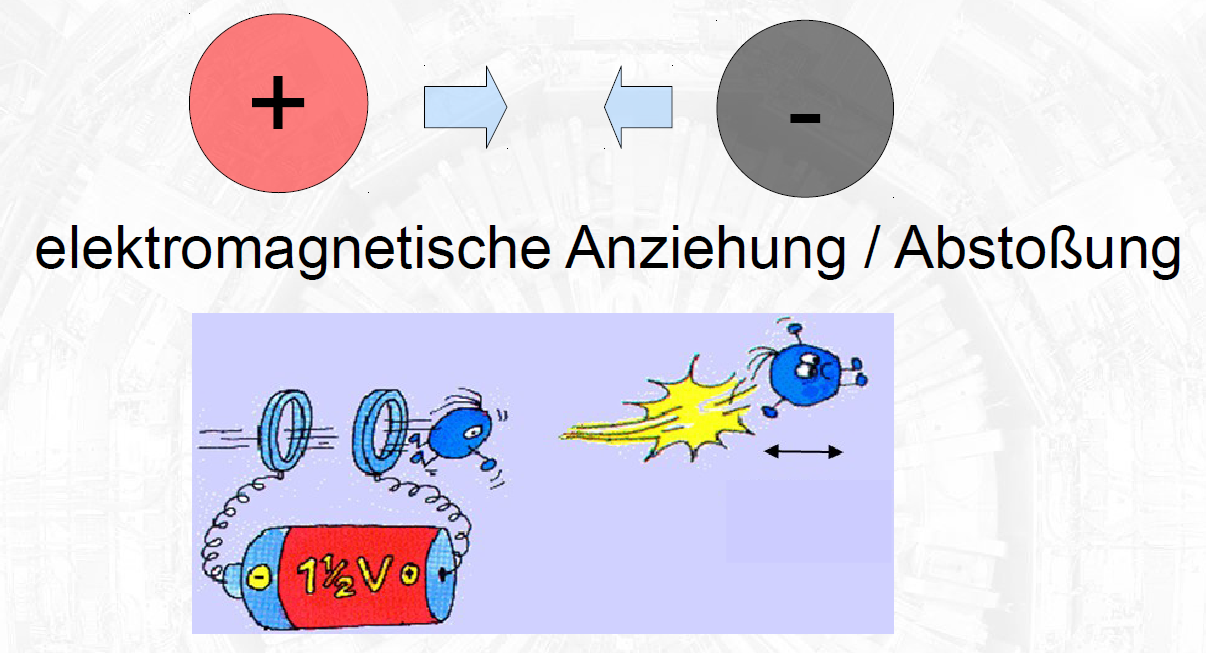
\includegraphics[width=0.65\textwidth]{lhc/Teilchenbeschleunigung.png}
  \end{center}
  \pause
  \begin{block}{Energieeinheit der Teilchenphysiker: Elektronenvolt \ev}
    $1\ev =$ Energie durch Beschleunigung mit Spannung von $1\,\text{V}$
    \visible<3->{
      \begin{itemize}
      \item<4-> Nach Batterie-Beschleunigung: \visible<5->{1,5\ev}
      \item<6-> Protonenmasse $\approx1\,000\,000\,000\ev = 1\gev$ ($1,7\cdot10^{-27}\kg$)
      \item<7-> \znull-Masse $\approx90\gev$
      \end{itemize}
    }
  \end{block}
\end{frame}

% --------------------------------------------------
\begin{frame}
  \frametitle{Beispiel f\"ur einen Teilchenbeschleuniger: R\"ohrenfernseher}
  \begin{center}
    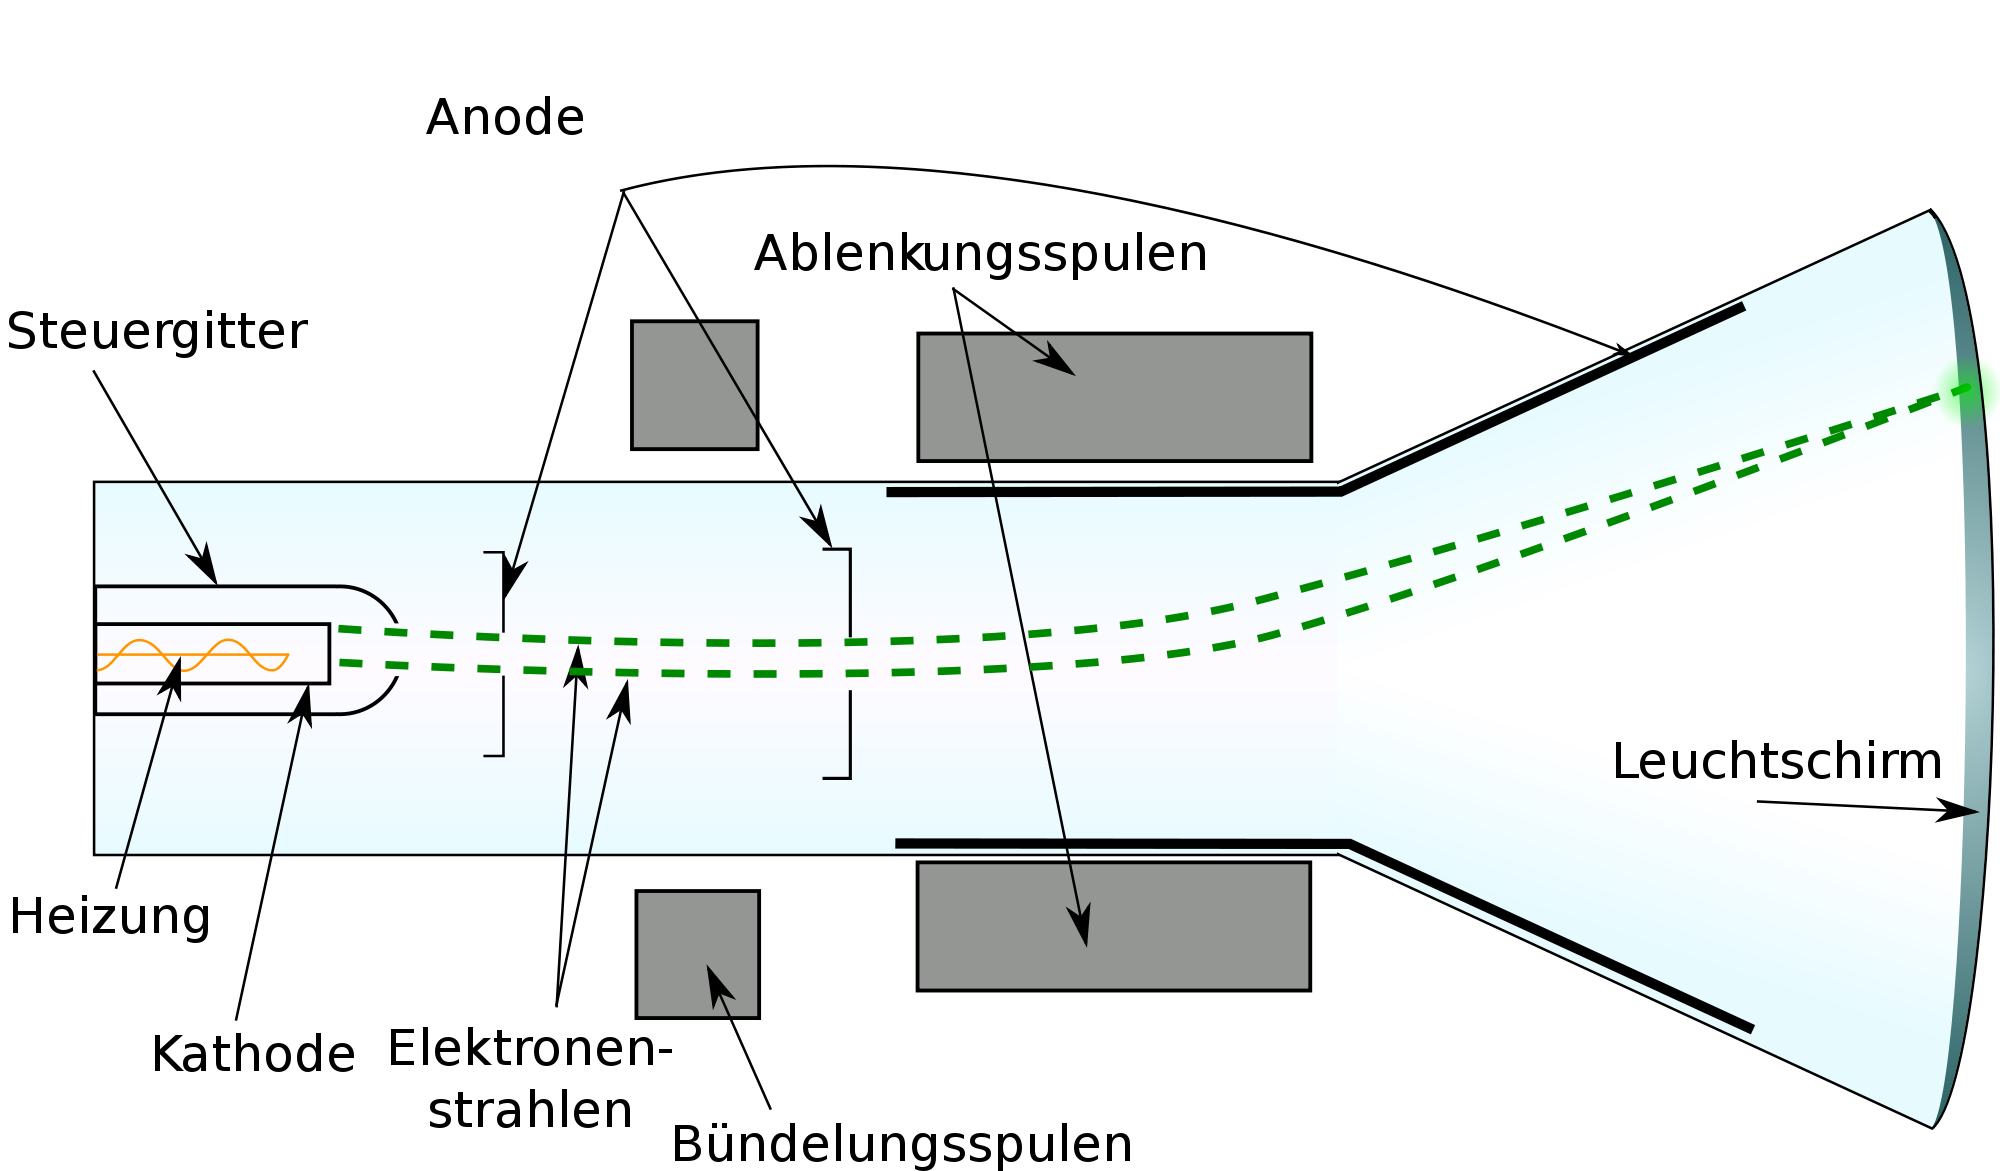
\includegraphics[width=0.7\textwidth]{lhc/2000px-Cathode_ray_tube_de.png}
  \end{center}
  \vskip1cm
  Spannung ca. 15\kev
\end{frame}

\section{LHC: Maschine der Superlative}
{
  \usebackgroundtemplate{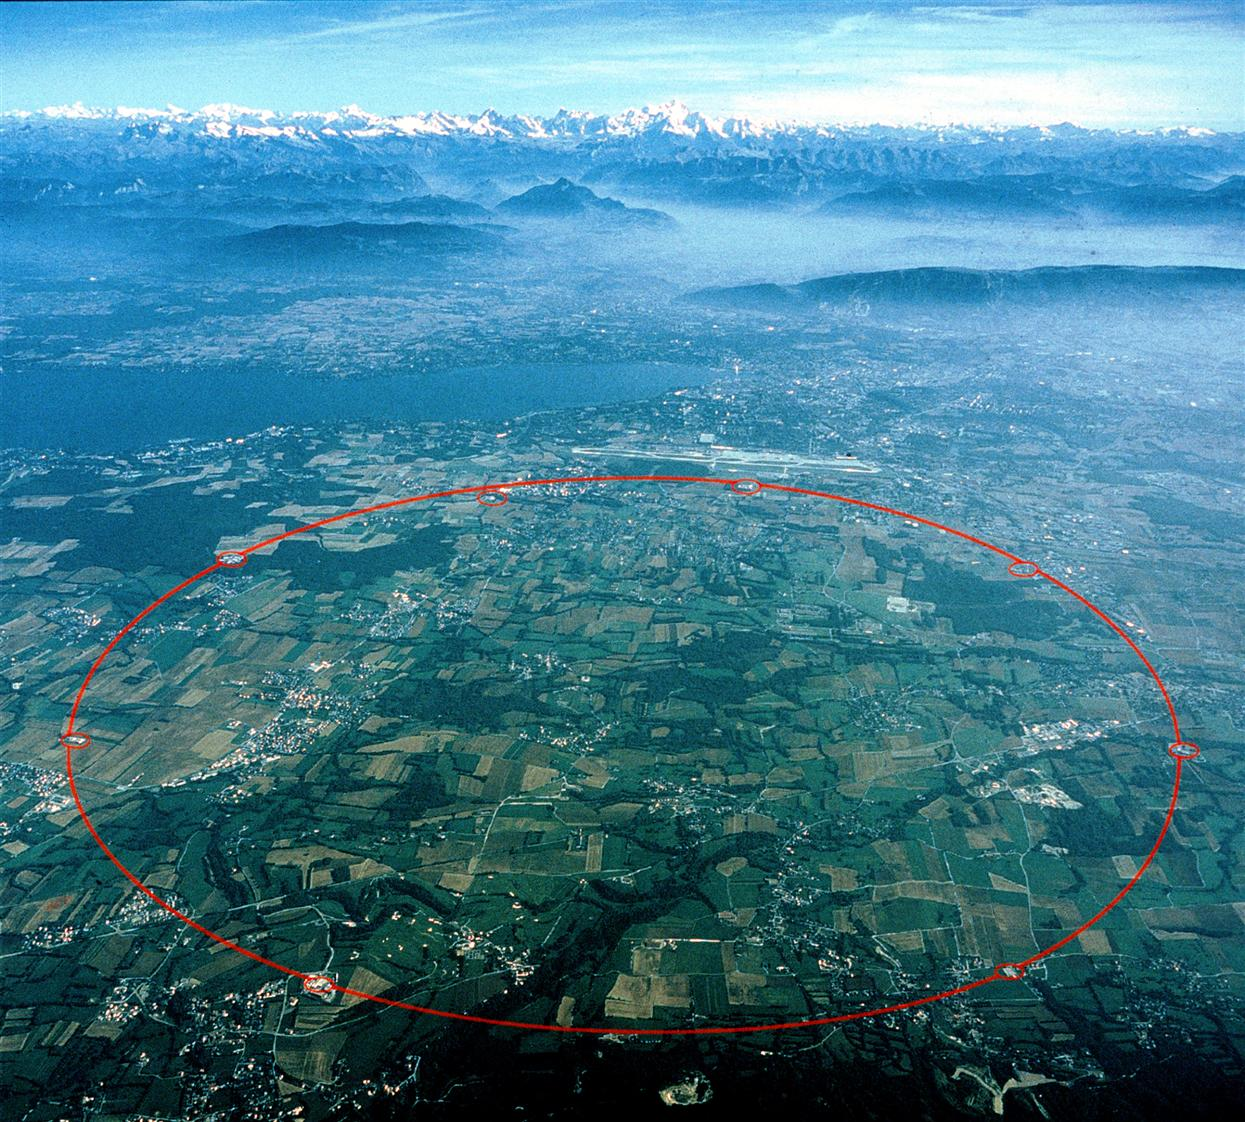
\includegraphics[width=\paperwidth]{lhc/LHC_0107014_01old-A4-at-144-dpi.jpg}}
  % --------------------------------------------------
  \begin{frame}
    \pause
    \begin{center}
      \begin{block}{Large Hadron Collider (LHC)}
        \begin{columns}
          \begin{column}{0.6\textwidth}
            \begin{itemize}
            \item Proton-Proton-Beschleuniger am CERN bei Genf
            \item Umfang von 27\km
            \item Zwischen 50 und 175\m unter der Erde
            \item[~] ~
            \end{itemize}
          \end{column}
          \begin{column}{0.4\textwidth}
            \vskip-0.5cm
            \centering
            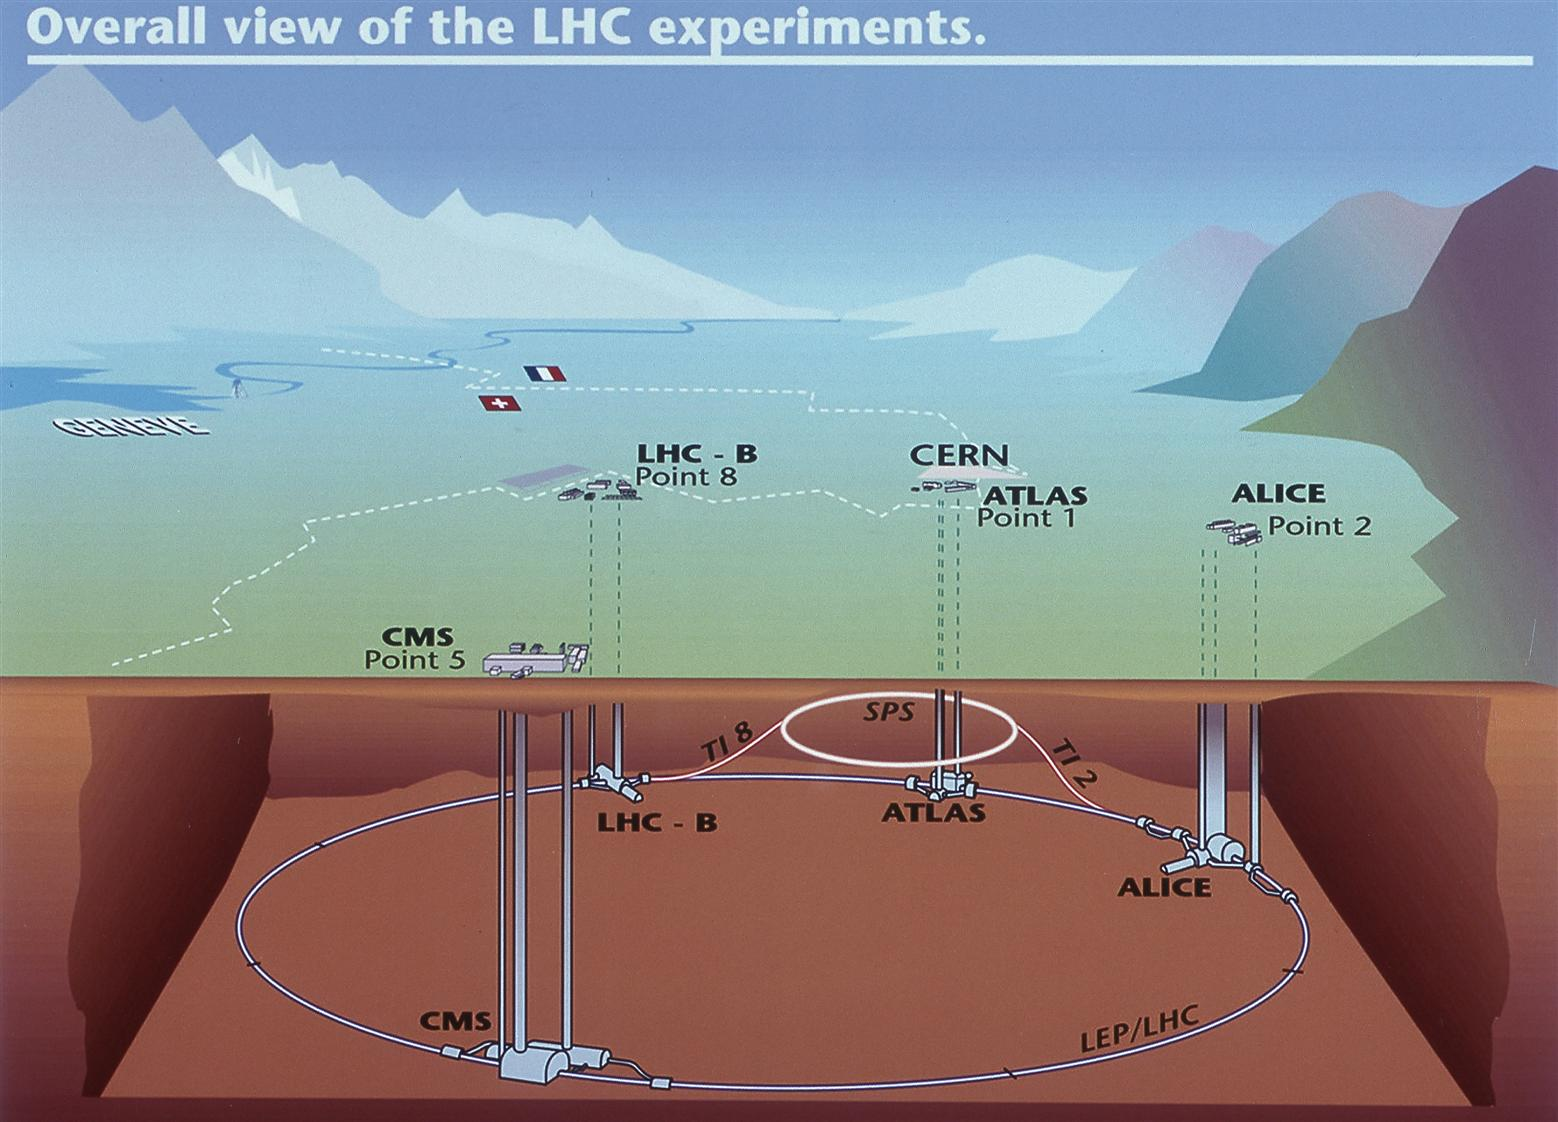
\includegraphics[width=0.9\textwidth]{lhc/LHC_9906026-A4-at-144-dpi.jpg}
          \end{column}
        \end{columns}
      \end{block}
   \end{center}
  \end{frame}

 % --------------------------------------------------
  \begin{frame}
    \frametitle{LHC: Der st\"arkste Beschleuniger der Welt}
    \begin{columns}
      \begin{column}{0.5\textwidth}
        \centering
      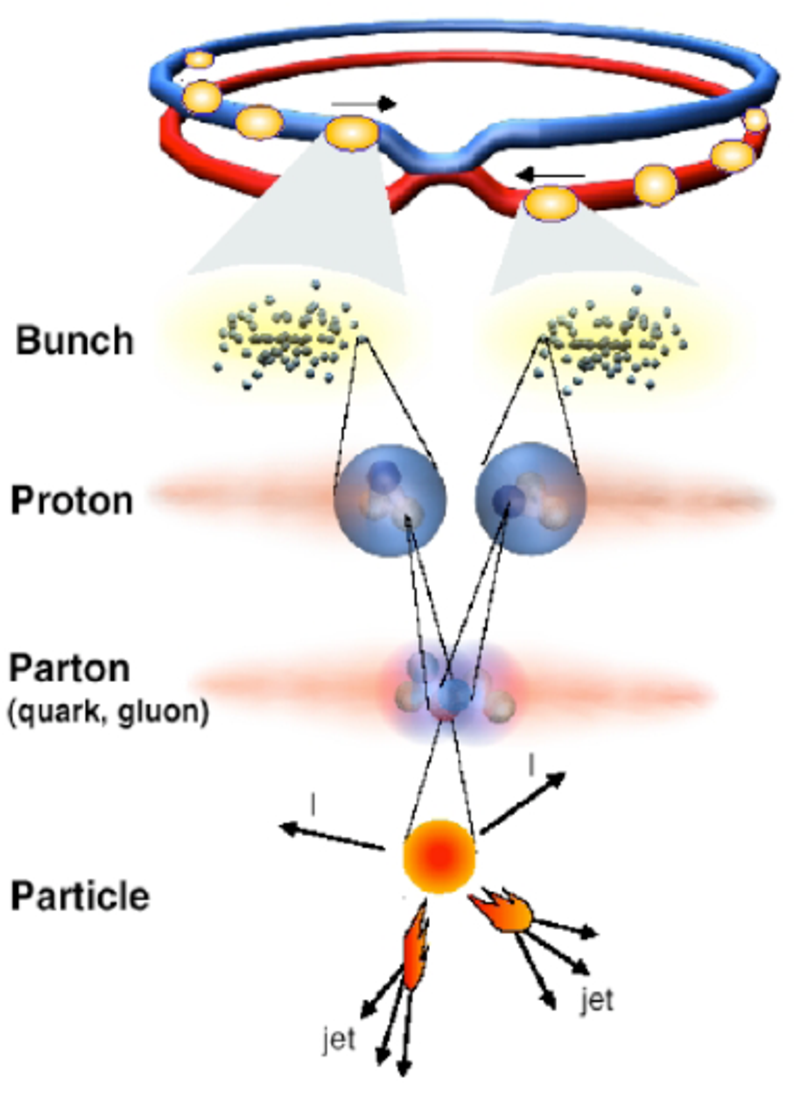
\includegraphics[width=0.9\textwidth]{lhc/LHC_Kollision_Schema}
      \end{column}
      \begin{column}{0.5\textwidth}
        \begin{block}{}
          \begin{itemize}
          \item Zwei gegenl\"aufige Strahlen
            \begin{itemize}
            \item 2\,808 ``Teilchenpakete''
            \item \ca 100 Milliarden Protonen pro Paket
            \end{itemize}
          \item Protonen beschleunigt durch elektrische Wechselfelder
            \begin{itemize}
            \item \textit{99,9999991\% der Lichtgeschwindigkeit}
            \item 11\,245 Uml\"aufe pro Sekunde
            \end{itemize}
          \end{itemize}
          \centering
          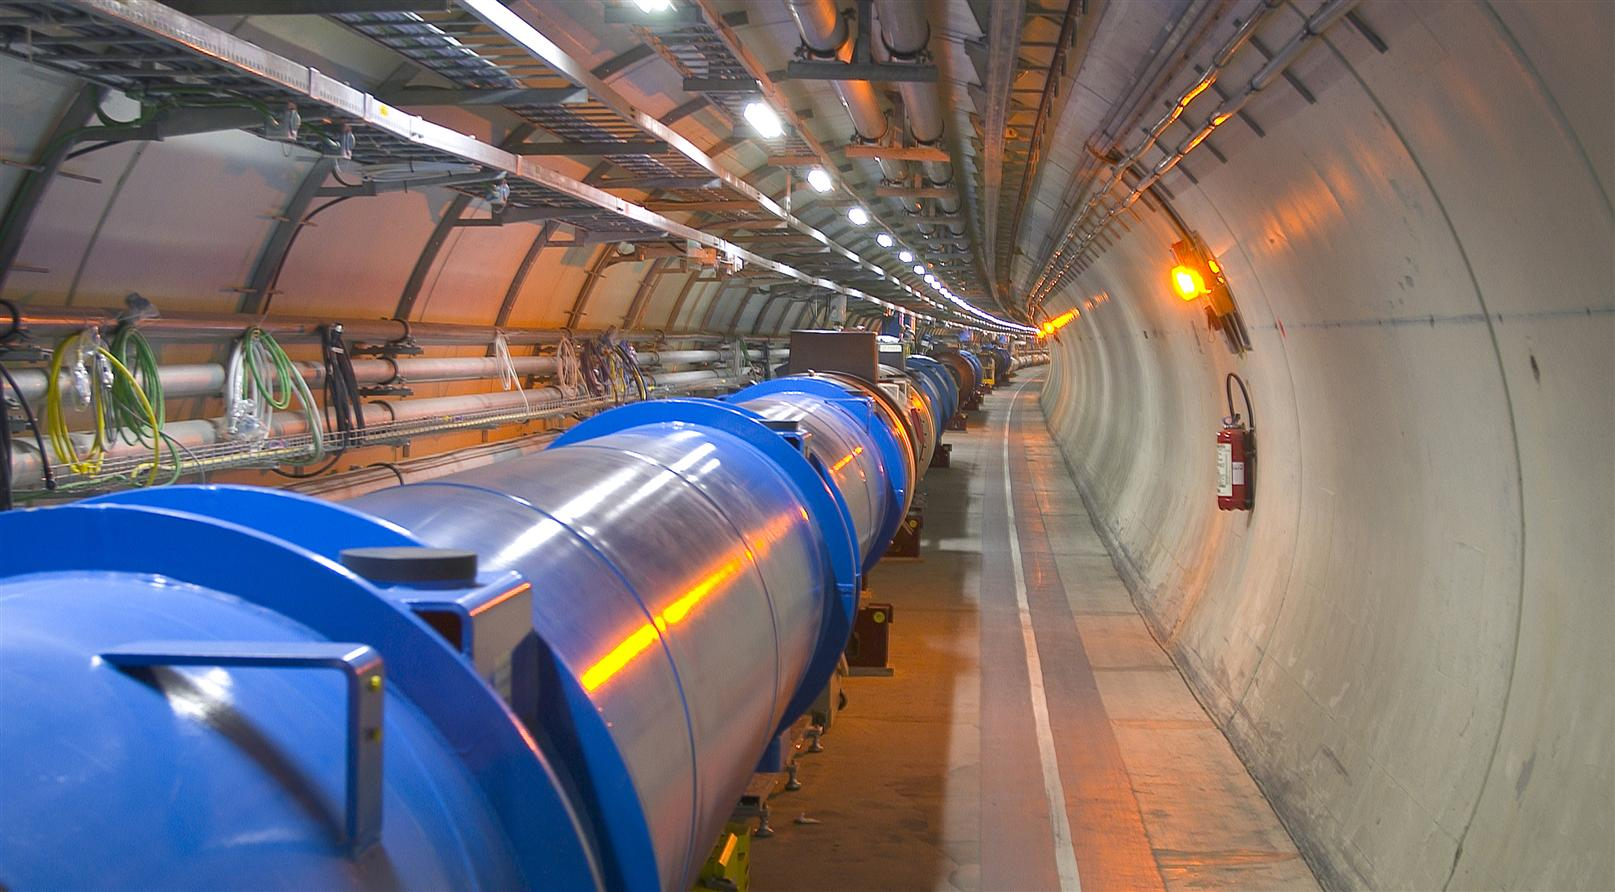
\includegraphics[width=0.8\textwidth]{lhc/LHC_Tunnel_0504028_01-A4-at-144-dpi.jpg}
        \end{block}
      \end{column}
    \end{columns}
  \end{frame}

  % --------------------------------------------------
  \begin{frame}
    \frametitle{LHC: K\"alter als das Weltall}
    \begin{columns}
      \begin{column}{0.5\textwidth}
        \centering
      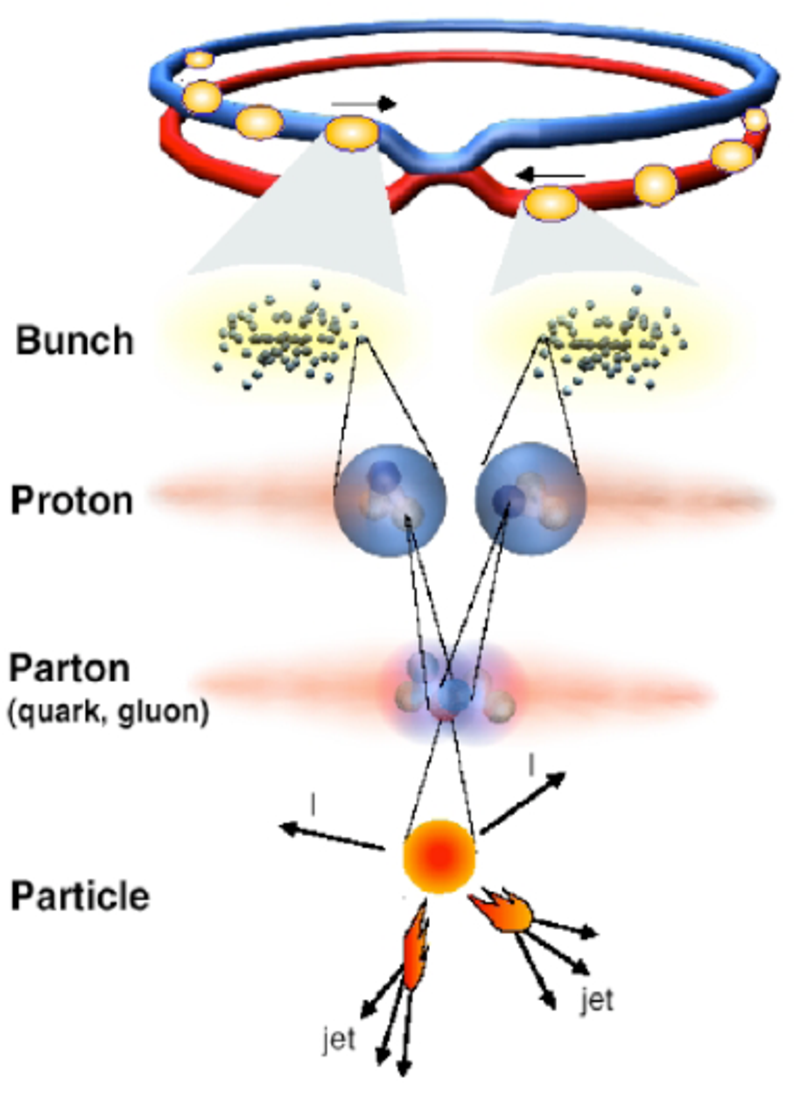
\includegraphics[width=0.9\textwidth]{lhc/LHC_Kollision_Schema}
      \end{column}
      \begin{column}{0.5\textwidth}
        \begin{block}{}
          \begin{itemize}
          \item Supraleitende Magnete zwingen Protonen auf Kreisbahn
            \begin{itemize}
            \item \textit{80\,000 mal st\"arker als Erdmagnetfeld}
            \end{itemize}
          \item Erfordern K\"uhlung auf 1,9\kelvin ($-271,3^{\circ}\,\text{C}$)
            \begin{itemize}
            \item \textit{K\"alter als das Weltall
              (2,7\kelvin)}
            \end{itemize}
          \end{itemize}
          \centering
          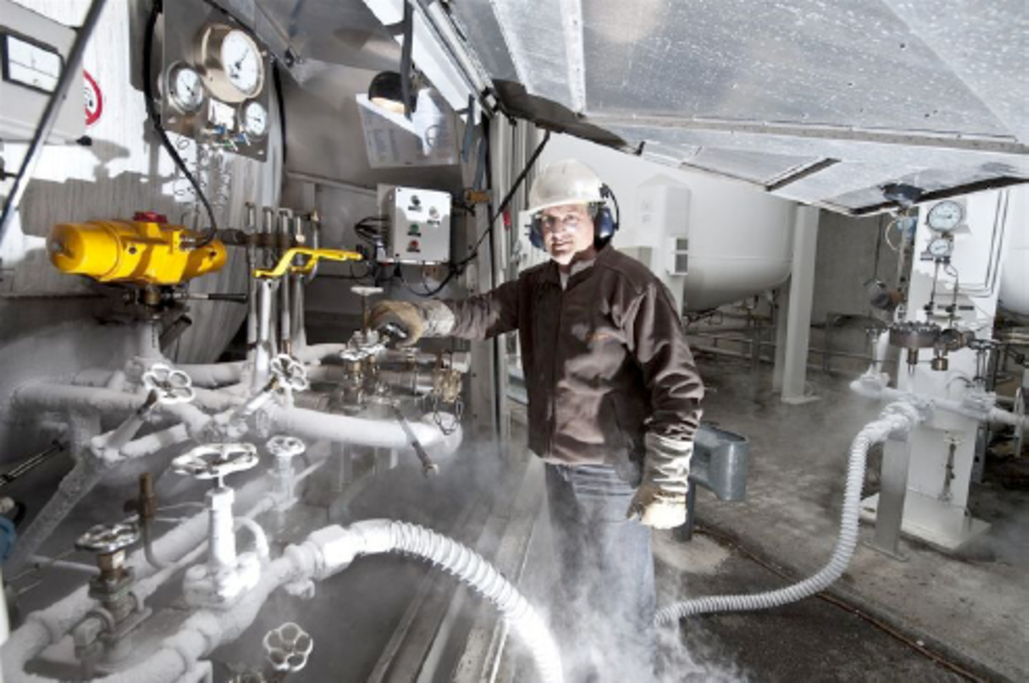
\includegraphics[width=0.8\textwidth]{lhc/LHC_Cryo}
        \end{block}
      \end{column}
    \end{columns}
  \end{frame}

  % --------------------------------------------------
  \begin{frame}
    \frametitle{LHC: Hei\ss{}er als die Sonne}
    \begin{columns}
      \begin{column}{0.5\textwidth}
        \centering
      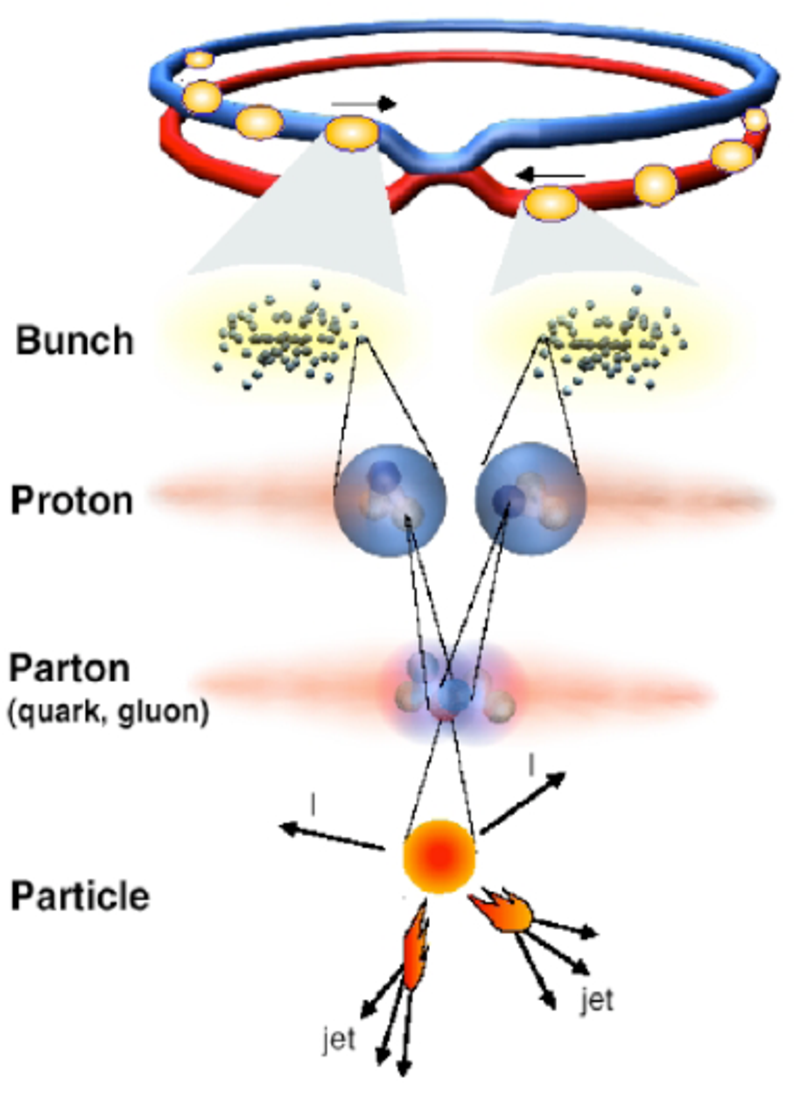
\includegraphics[width=0.9\textwidth]{lhc/LHC_Kollision_Schema}
      \end{column}
      \begin{column}{0.5\textwidth}
        \begin{block}{}
          \begin{itemize}
          \item \ca 400 Millionen Kollisionen pro Sekunde
          \item Energie von 7\tev $\approx80\,m_{Z^{0}}$
            \begin{itemize}
            \item \textit{100\,000 mal hei\ss{}er als im Innern der Sonne}
            \end{itemize}
          \end{itemize}
          \centering
          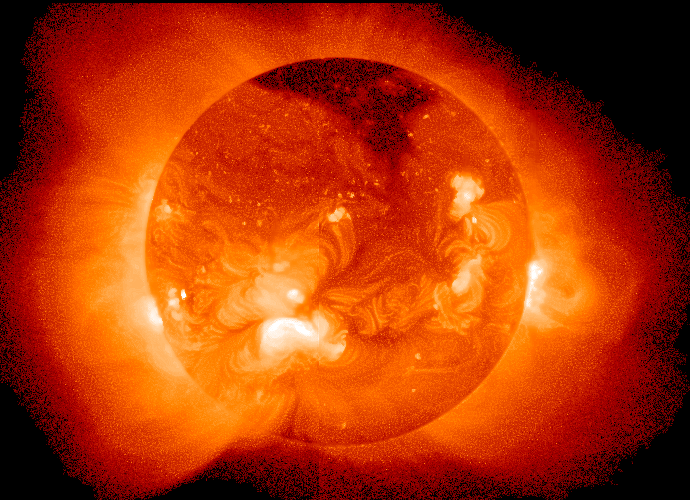
\includegraphics[width=0.8\textwidth]{lhc/Sun_in_X-Ray}
        \end{block}
      \end{column}
    \end{columns}
  \end{frame}

  % --------------------------------------------------
  \begin{frame}
    \frametitle{LHC: Proton-Proton Kollision}
    \begin{columns}
      \begin{column}{0.5\textwidth}
        \centering
      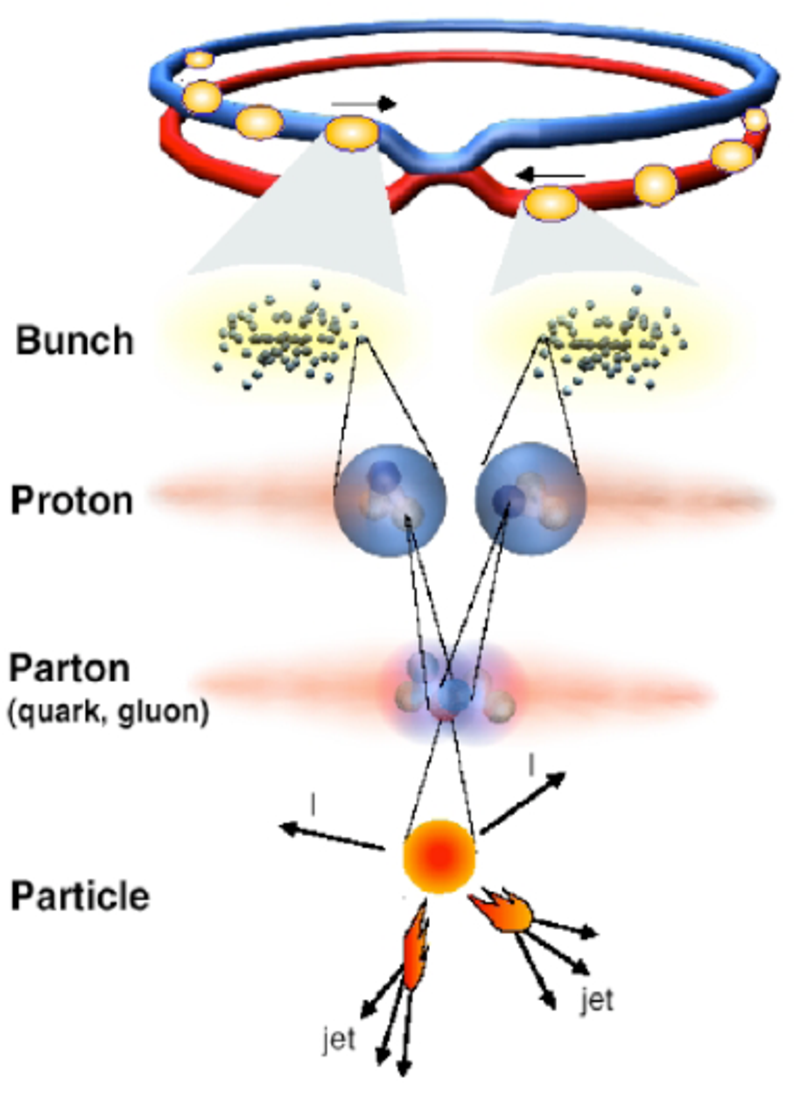
\includegraphics[width=0.9\textwidth]{lhc/LHC_Kollision_Schema}
      \end{column}
      \begin{column}{0.5\textwidth}
        \begin{block}{}
          \centering
          \texttt{\scriptsize www.youtube.com/watch?v=RdYvtm4CIAE}
        \end{block}
      \end{column}
    \end{columns}
  \end{frame}

  % --------------------------------------------------
  \begin{frame}
    \frametitle{LHC: Proton-Proton Kollision}
    \begin{center}
      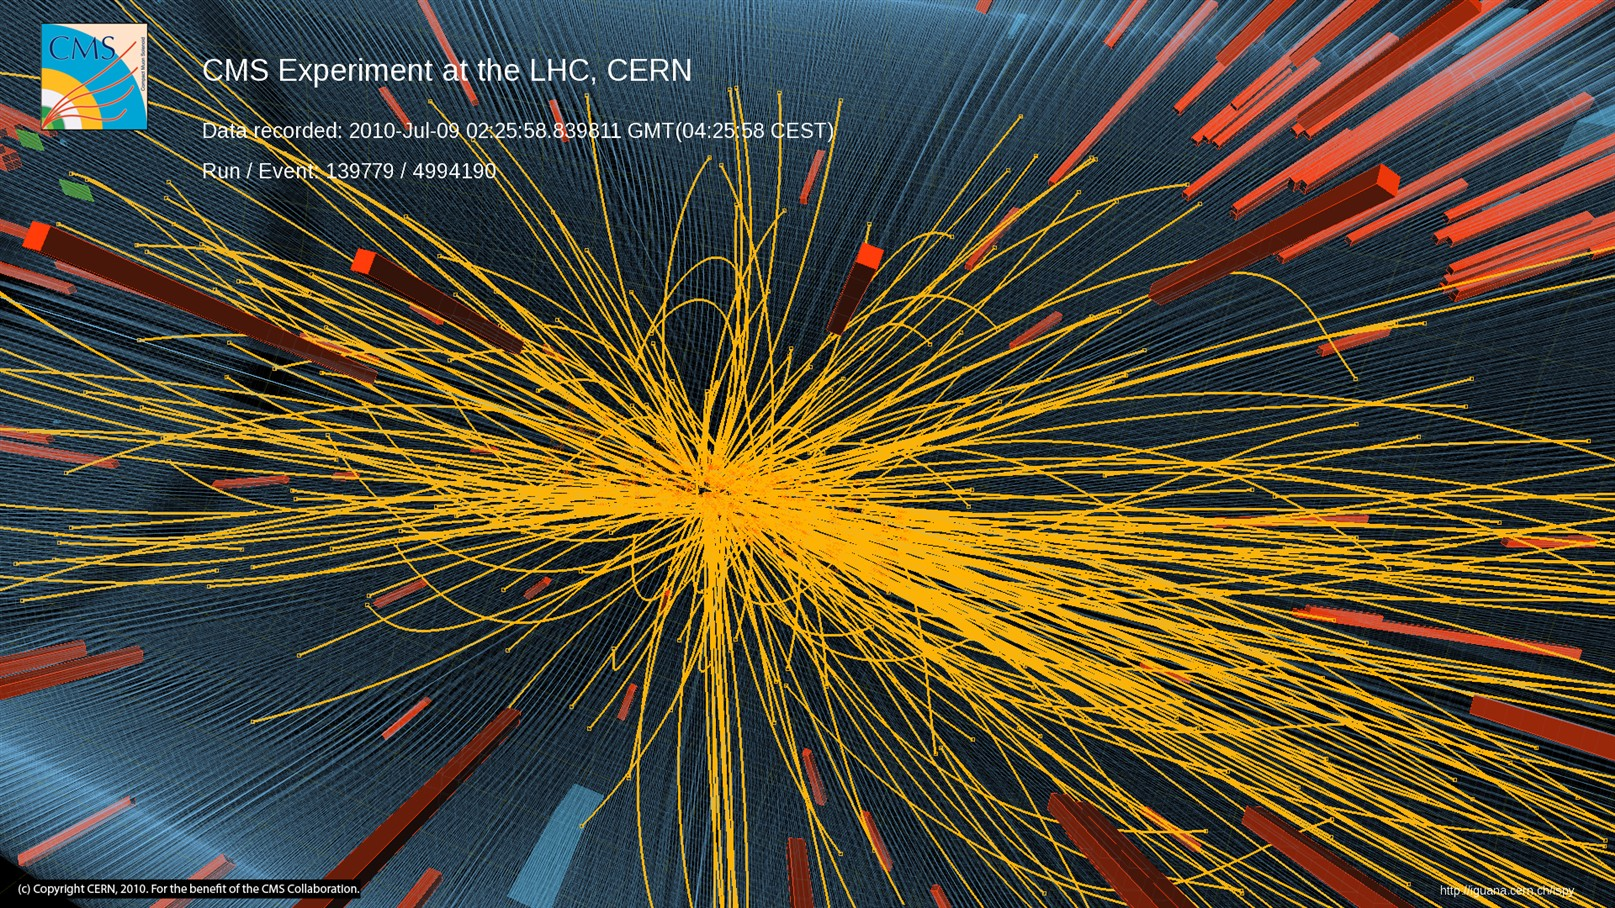
\includegraphics[width=0.95\textwidth]{lhc/CMS-Event.jpg}
    \end{center}
  \end{frame}


  \section{Nachweis von Elementarteilchen}
  \subsection{Teilchendetektoren}
  % --------------------------------------------------
  \begin{frame}
    \frametitle{Wie misst man das??}
    \begin{center}
      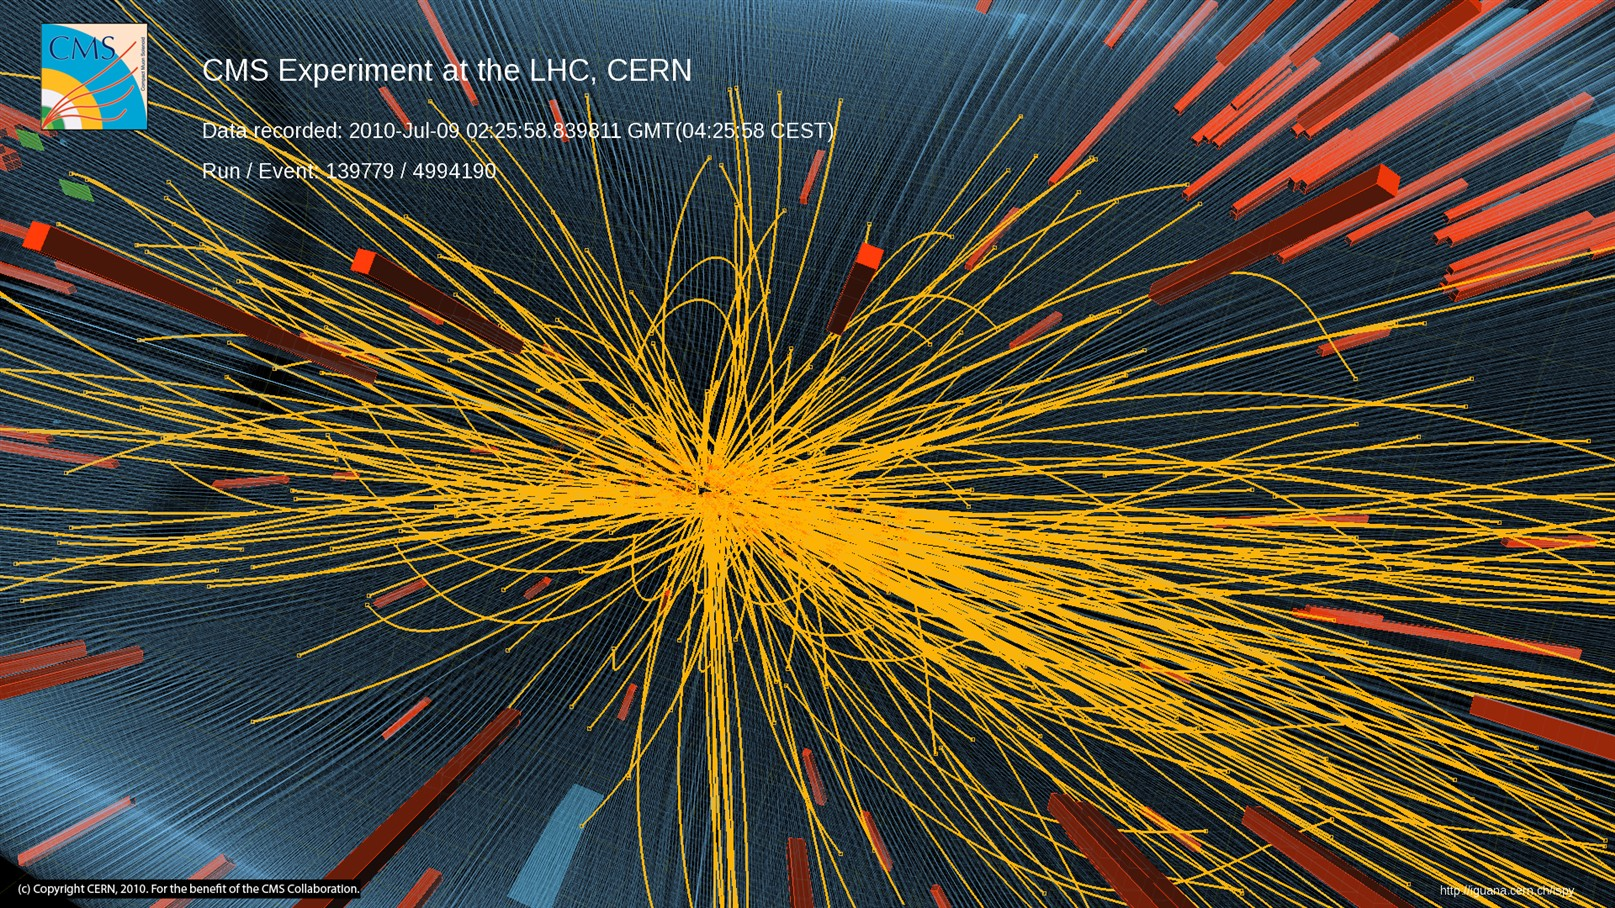
\includegraphics[width=0.95\textwidth]{lhc/CMS-Event.jpg}
    \end{center}
  \end{frame}
}

% --------------------------------------------------
\begin{frame}
  \frametitle{Detektoren: Teilchen ``sehen''}
  \begin{columns}
    \visible<3->{
      \begin{column}{0.3\textwidth}
        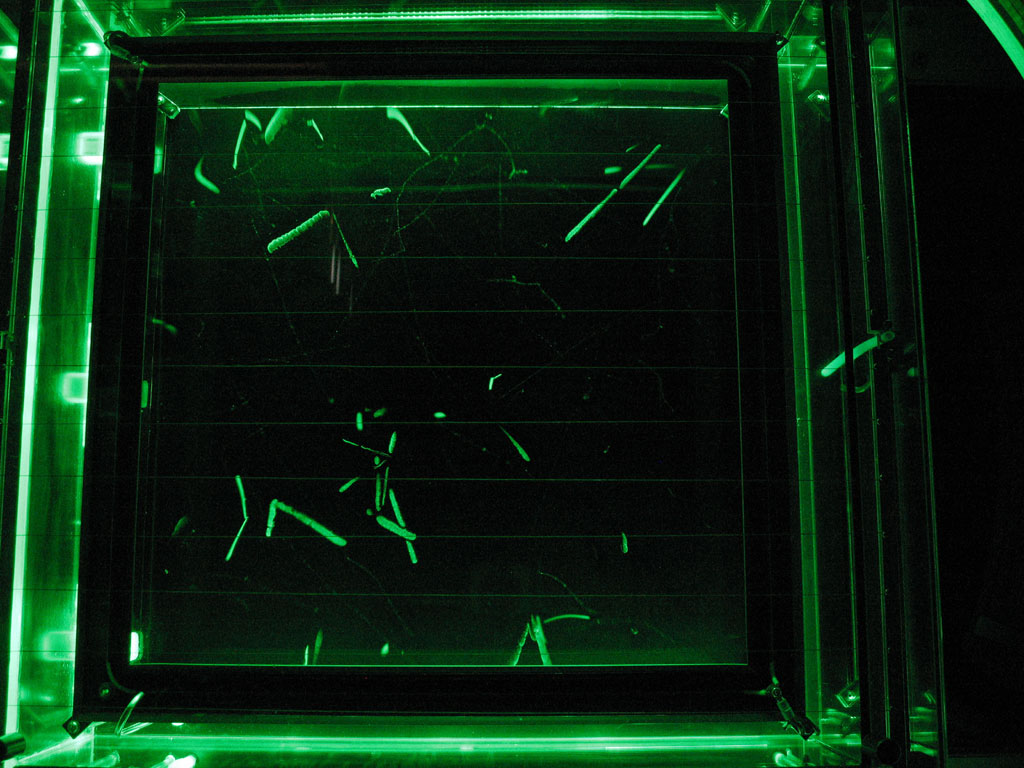
\includegraphics[width=0.98\textwidth]{lhc/DESYNebelkammer.jpg}
      \end{column}     
    }
    \visible<4->{
      \begin{column}{0.3\textwidth}
        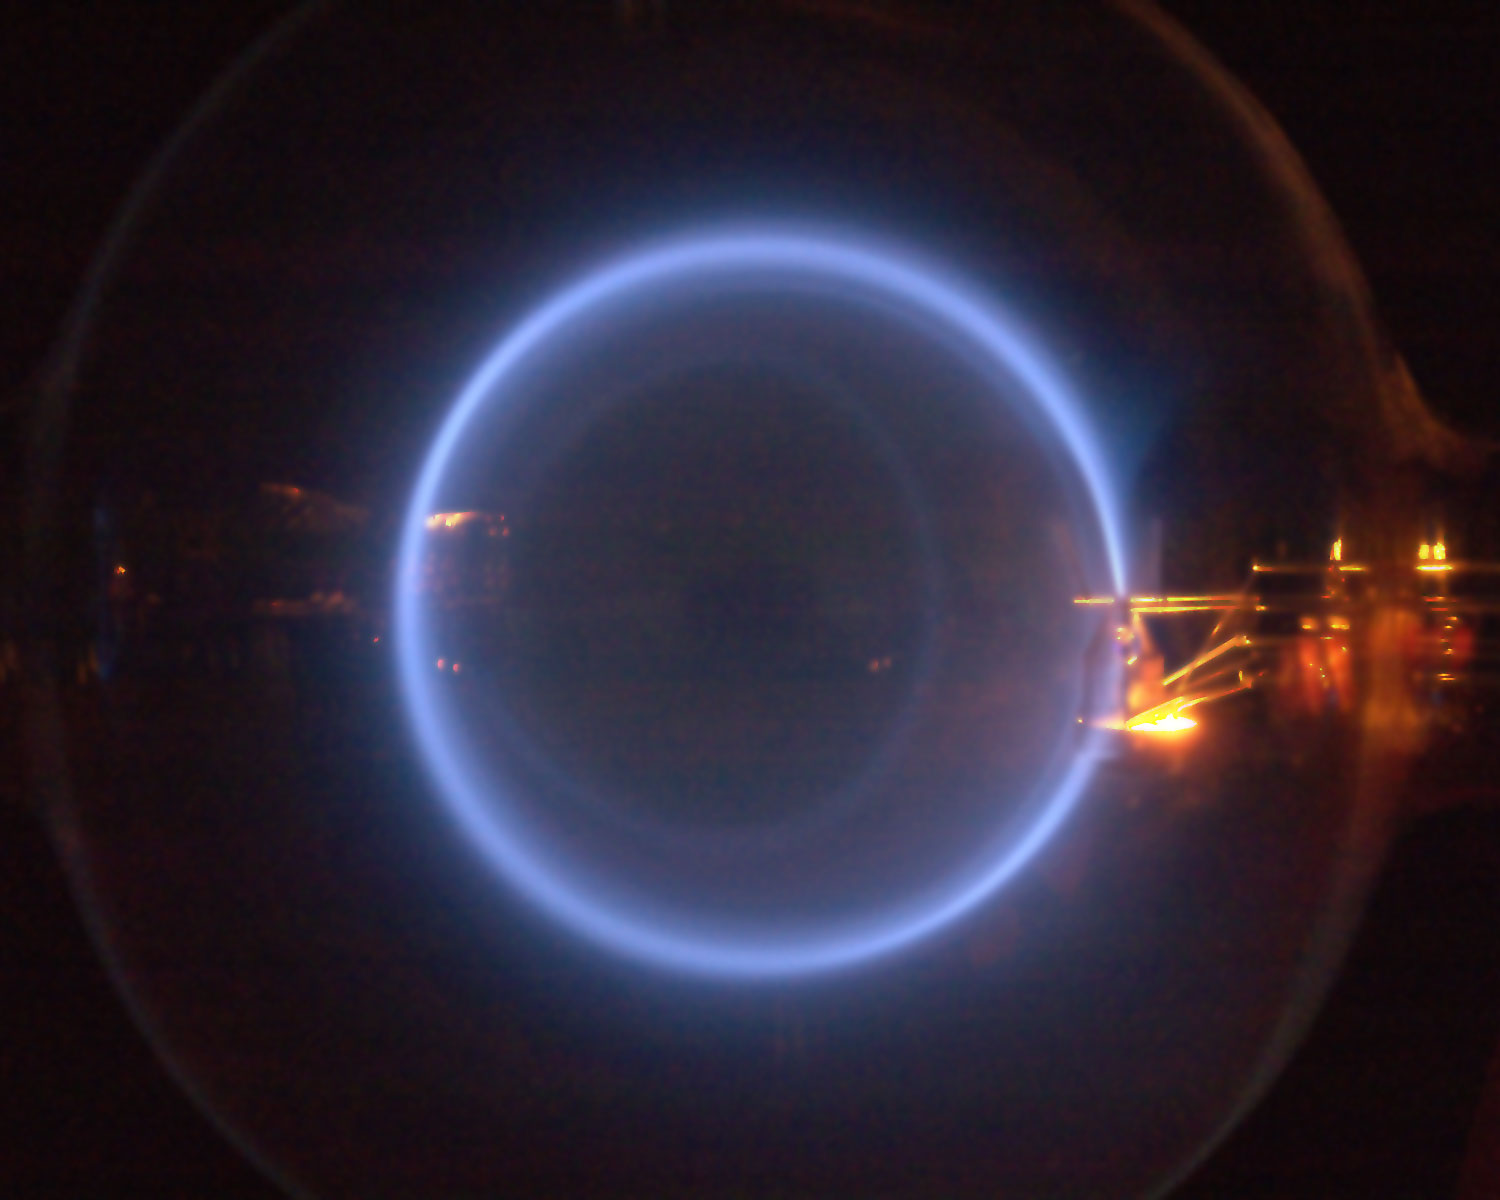
\includegraphics[width=0.98\textwidth]{lhc/Fadenstrahlrohr.jpg}
      \end{column}     
    }
    \visible<5->{
      \begin{column}{0.3\textwidth}
        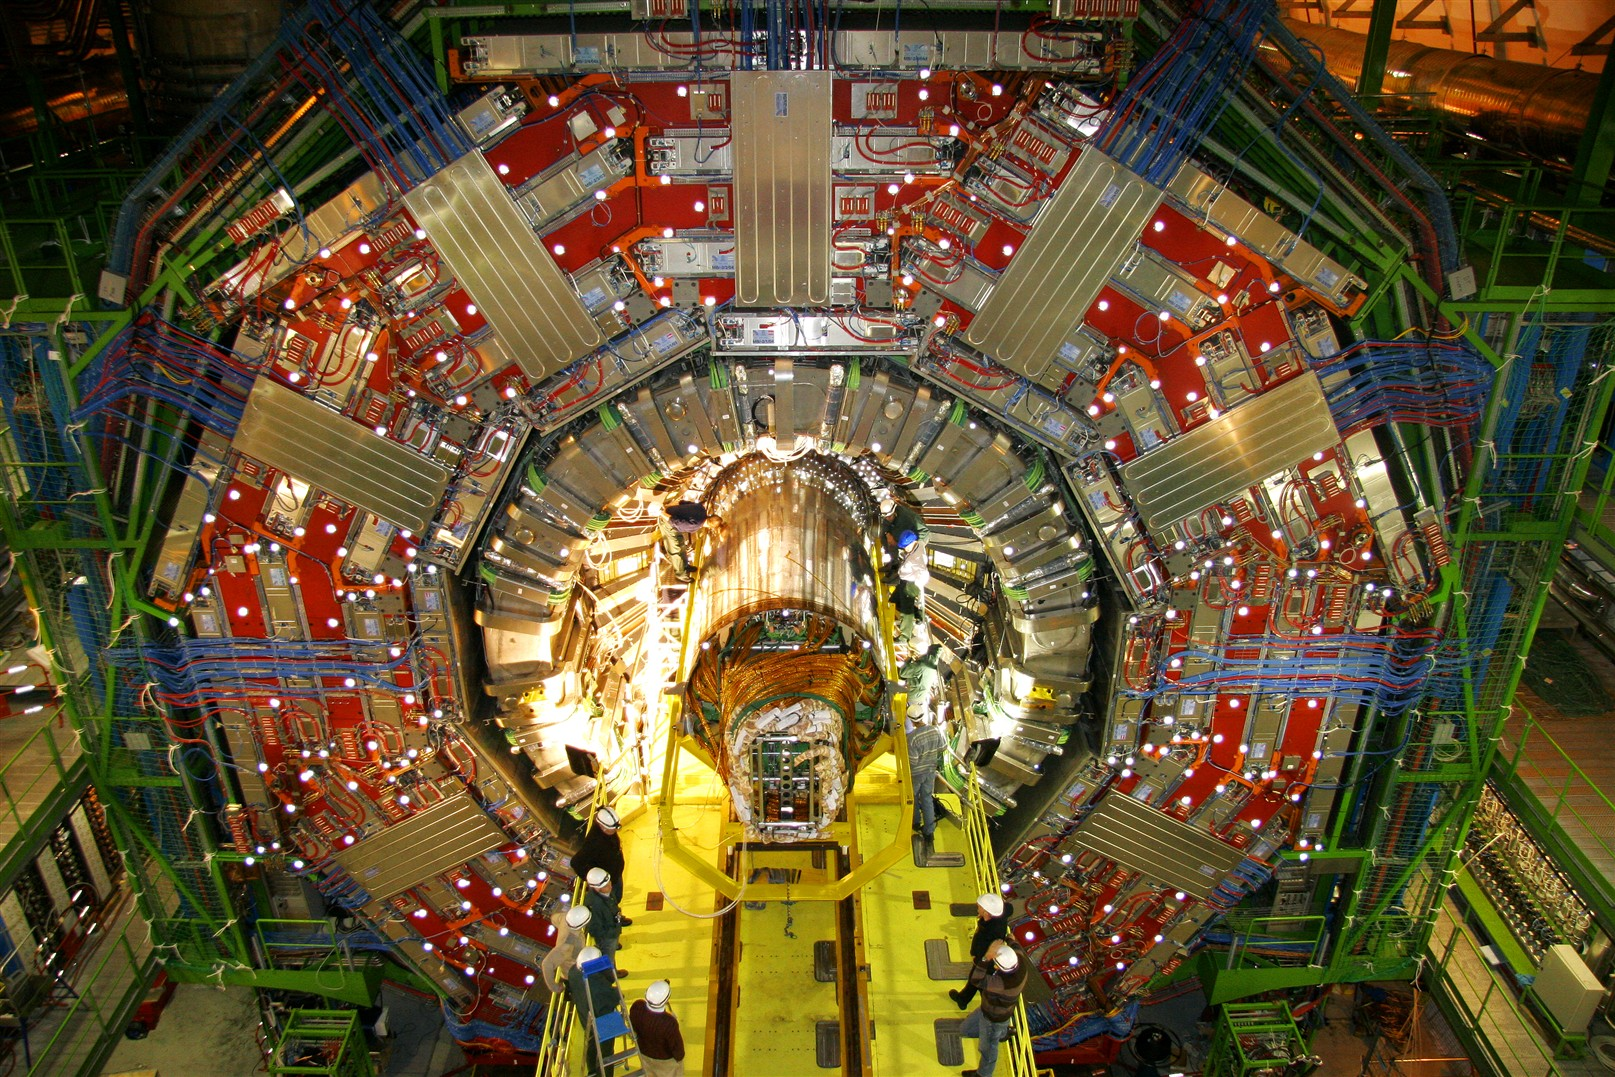
\includegraphics[width=\textwidth]{lhc/CMS_0712023_01-A4-at-144-dpi.jpg}
      \end{column}     
    }
    \end{columns}
    \vskip1cm
    \begin{center}
      \visible<2->{\Large Teilchen wechselwirken mit Materie
      $\rightarrow$ messbares Signal
    }
  \end{center}
\end{frame}
   
% --------------------------------------------------
\begin{frame}
  \frametitle{Wenn Teilchen auf Materie treffen\ldots}
  \begin{columns}[T]
    \begin{column}{0.65\textwidth}
      \begin{itemize}
      \item<2-> Geladene Teilchen: Ionisation
      \end{itemize}
      \begin{columns}[T]
        \begin{column}{0.4\textwidth}
          \centering
          \visible<2->{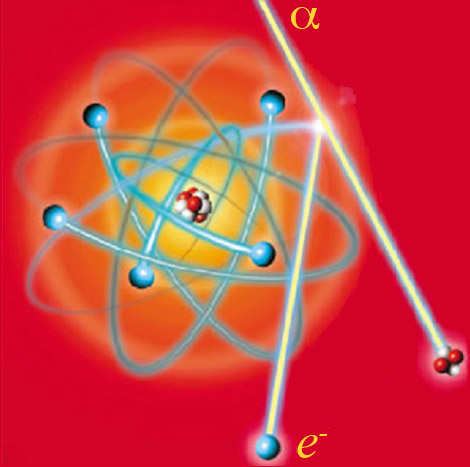
\includegraphics[width=0.9\textwidth]{lhc/ionisation_atome.jpg}}
        \end{column}
        \begin{column}{0.6\textwidth}
          \begin{itemize}
          \item<2-> \textbf{Freie Ladungstr\"ager}
            \begin{itemize}
            \item<3-> Nebelkammer\\$\rightarrow$\emph{``Kondensstreifen''}
            \item<4-> Siliziumdetektor\\$\rightarrow$\emph{Strompuls}
            \end{itemize}
          \end{itemize}
        \end{column}
      \end{columns}
      \begin{itemize}
      \item<5-> Geladene \& neutrale Teilchen: abgestoppt
      \end{itemize}
      \begin{columns}[T]
        \begin{column}{0.4\textwidth}
          \centering
          \visible<5->{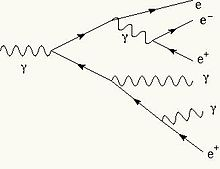
\includegraphics[width=\textwidth]{lhc/220px-Schematic_of_a_particle_shower.jpg}}
        \end{column}
        \begin{column}{0.6\textwidth}
          \begin{itemize}
          \item<5-> \textbf{Teilchenschauer}
            \begin{itemize}
            \item<6-> Kalorimeter\\$\rightarrow$\emph{Lichtblitze}
            \end{itemize}
          \end{itemize}
        \end{column}
      \end{columns}
    \end{column}
    \begin{column}{0.35\textwidth}
      \centering
      \visible<3->{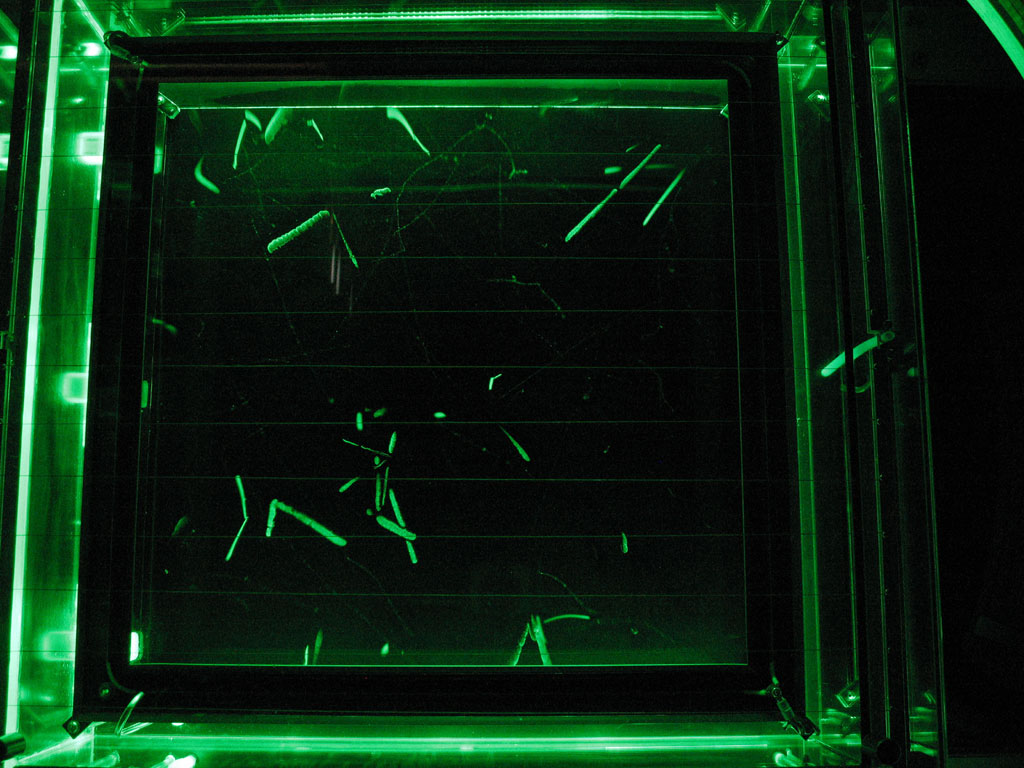
\includegraphics[width=0.8\textwidth]{lhc/DESYNebelkammer.jpg}}\\
      \visible<4->{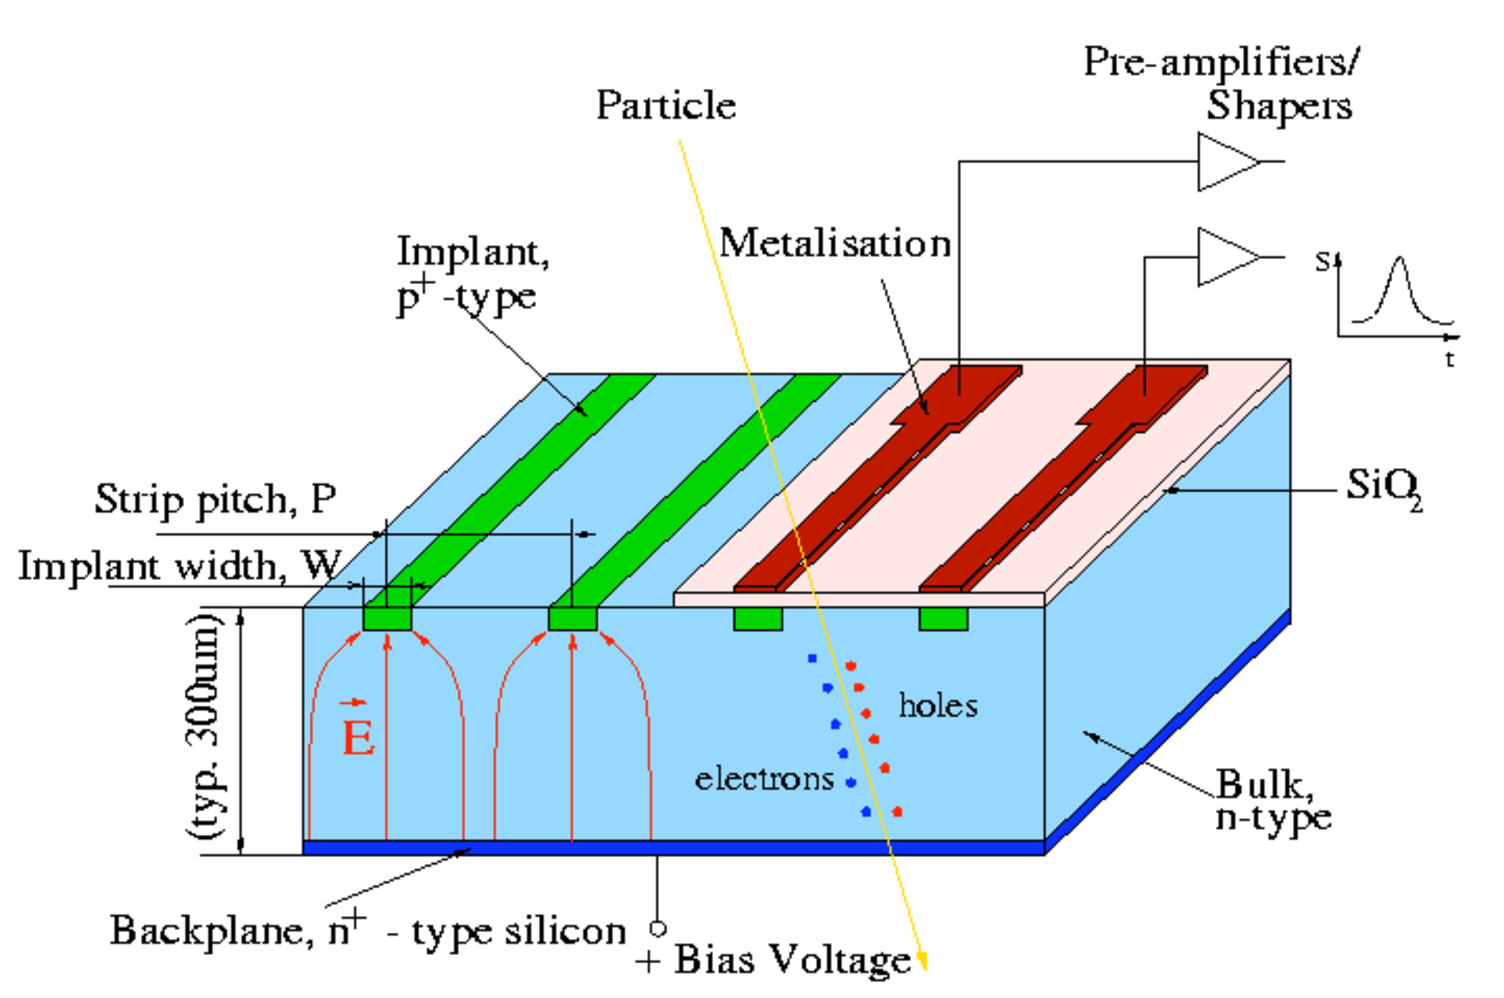
\includegraphics[width=\textwidth]{lhc/Silicon_Detector.pdf}}\\
      \visible<6->{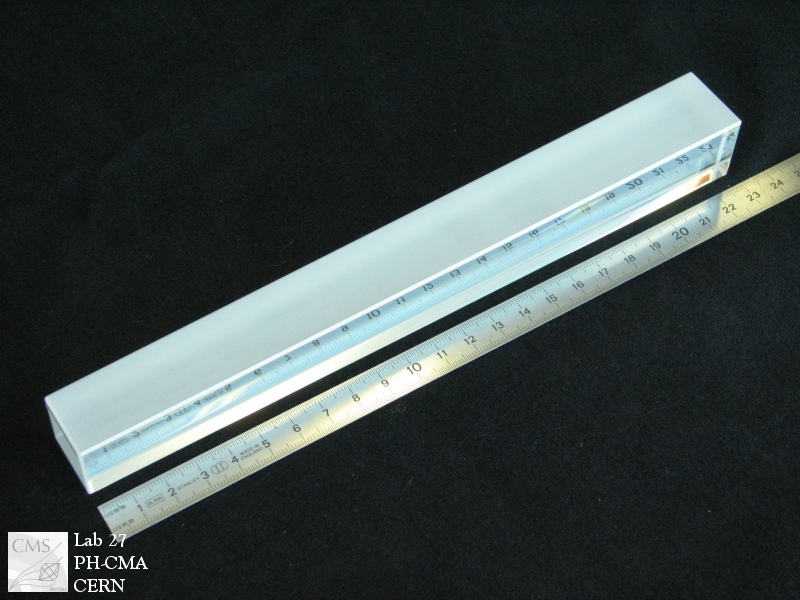
\includegraphics[width=0.7\textwidth]{lhc/CMS-Crystal.jpg}}
    \end{column}
  \end{columns}
\end{frame}


\subsection{Detektoren am LHC}
% --------------------------------------------------
\begin{frame}
  \frametitle{Die gro\ss{}en Detektoren am LHC}
  \begin{center}
    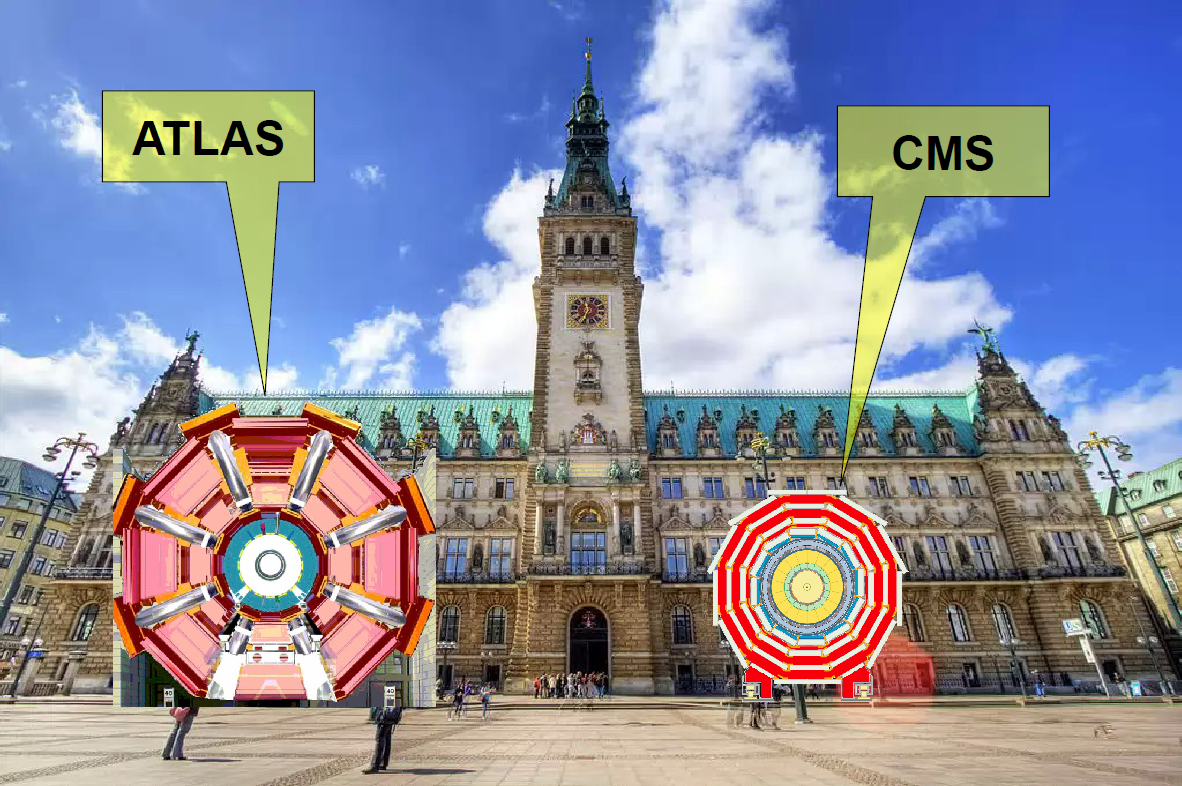
\includegraphics[width=0.95\textwidth]{lhc/ATLAS-CMS-RathausHH.png}
  \end{center}
\end{frame}

% --------------------------------------------------
\begin{frame}
  \frametitle{Der CMS-Detektor am LHC}
  \begin{columns}
    \begin{column}{0.6\textwidth}
      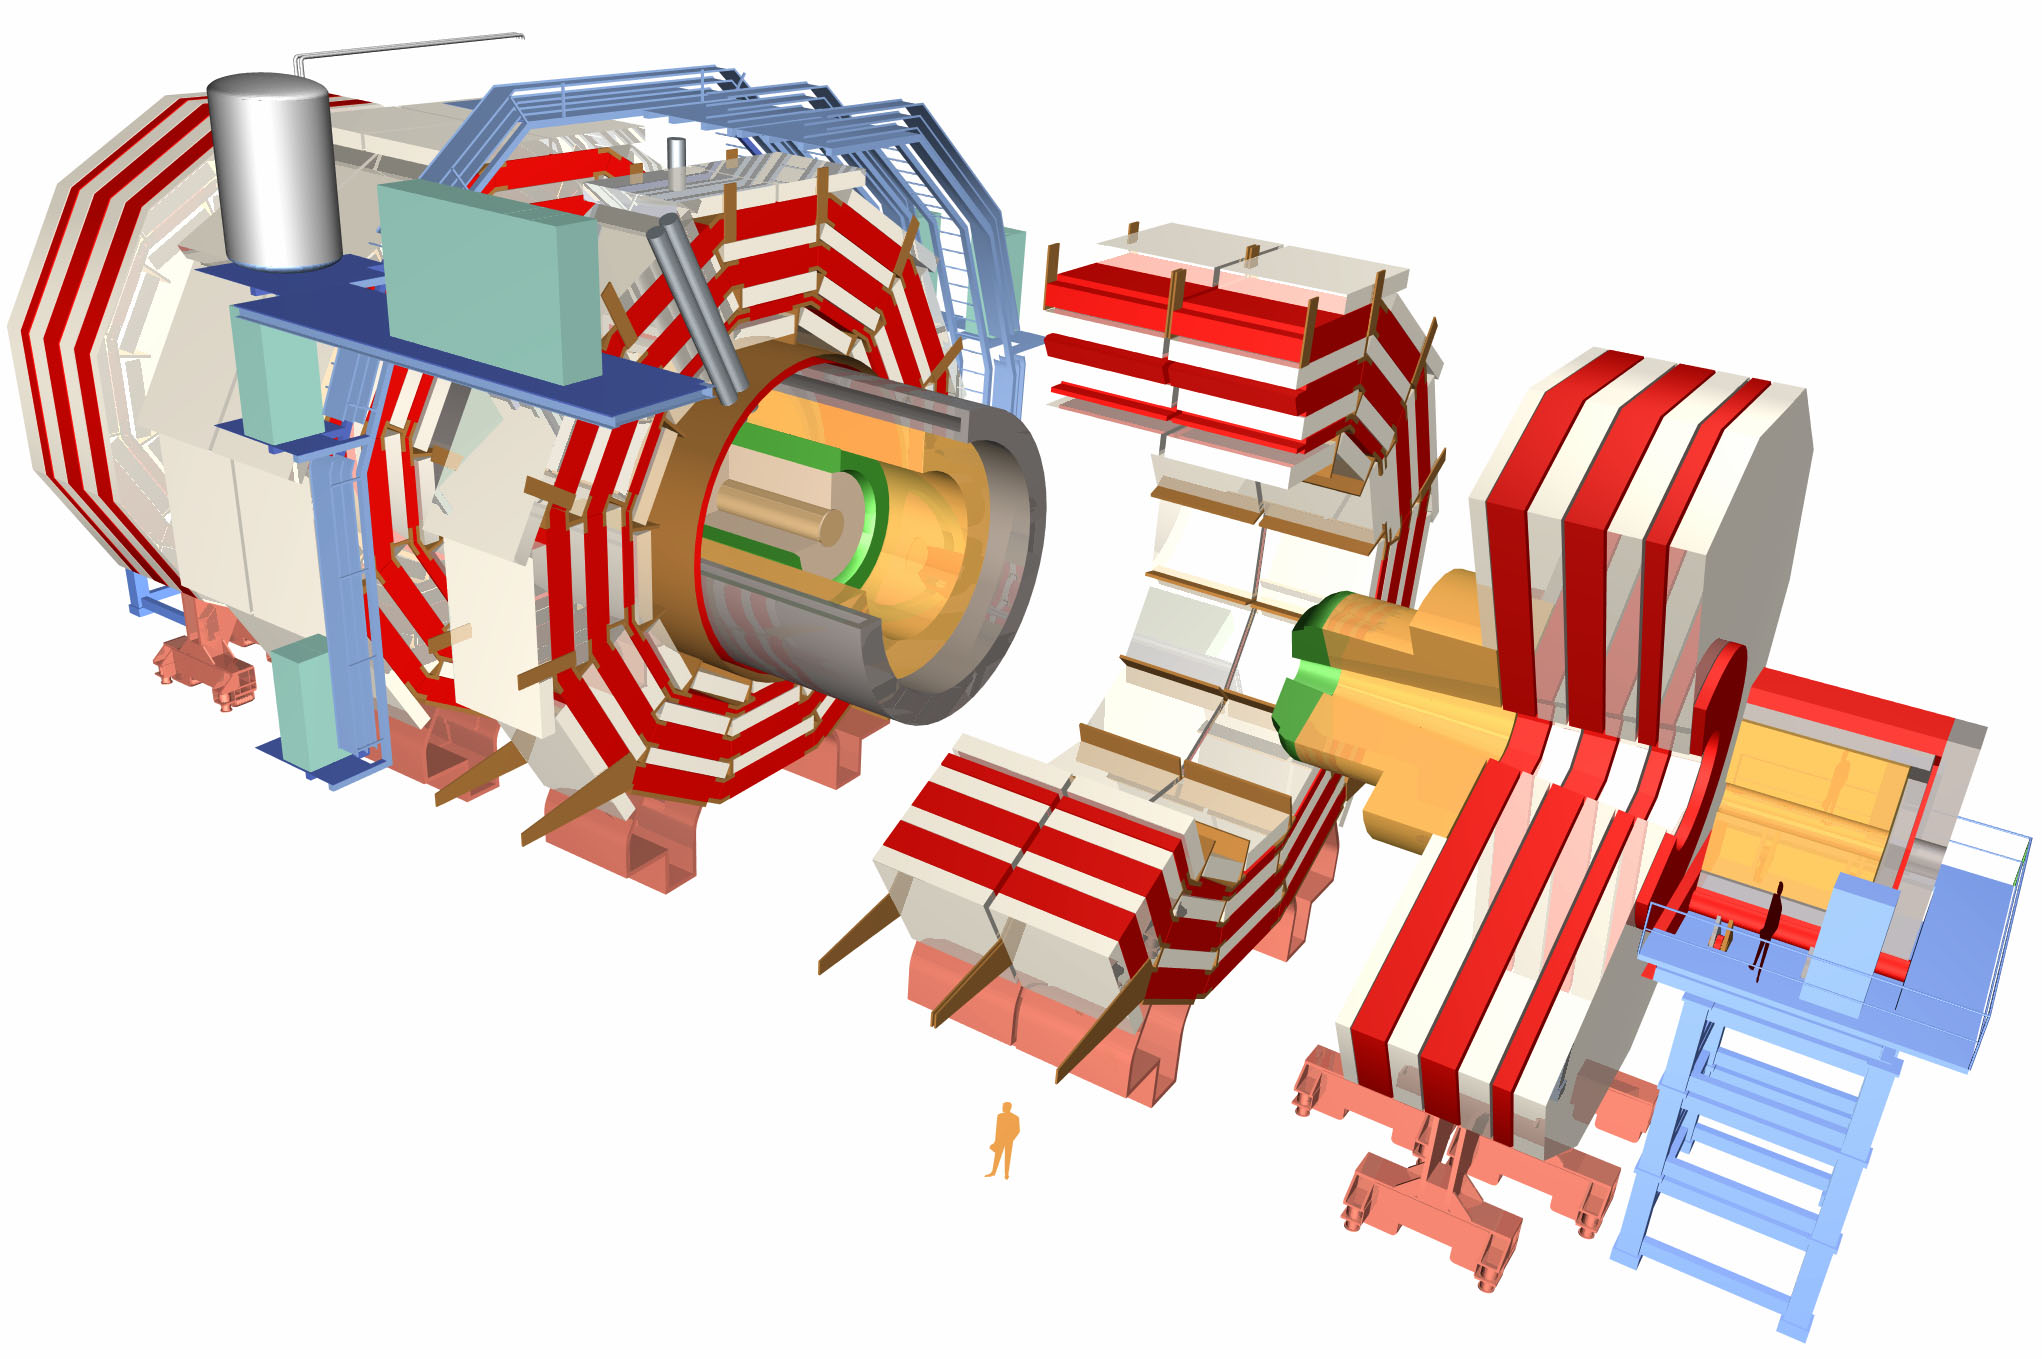
\includegraphics[width=0.95\textwidth]{lhc/CMSnc.jpg}
    \end{column}
    \begin{column}{0.4\textwidth}
      \begin{block}{}
        \begin{itemize}
        \item Breite: 15\m
        \item H\"ohe: 15\m
        \item L\"ange: 21\m
        \item Gewicht: 12\,500\tons
        \item Mehr als 3\,000 Wissenschaftler aus 38 L\"andern
        \end{itemize}
      \end{block}
    \end{column}
  \end{columns}
\end{frame}

% --------------------------------------------------
\begin{frame}[t]
  \frametitle{\only<1-2>{Was m\"ochte man von den Teilchen wissen?}\only<3->{Spurdetektor}}
  \vskip0.3cm
  \only<2-5>{
    \begin{columns}
      \begin{column}{0.18\textwidth}
        \begin{block}{}
          \centering
          Richtung
        \end{block}
      \end{column}
      \begin{column}{0.025\textwidth}
      \end{column}
      \begin{column}{0.18\textwidth}
        \begin{block}{}
          \centering
          Impuls        
        \end{block}
      \end{column}
      \begin{column}{0.025\textwidth}
      \end{column}
      \begin{column}{0.18\textwidth}
        \begin{block}{}
          \centering
          Ladung
        \end{block}
      \end{column}
      \begin{column}{0.025\textwidth}
      \end{column}
      \begin{column}{0.18\textwidth}
        \begin{block}{}
          \centering
          Energie
        \end{block}
      \end{column}
      \begin{column}{0.02\textwidth}
      \end{column}
      \begin{column}{0.18\textwidth}
        \begin{block}{}
          \centering
          \textcolor{white}{g}Teilchenart\textcolor{white}{g}
        \end{block}
      \end{column}
      \begin{column}{0.005\textwidth}
      \end{column}
    \end{columns}
  }
  \only<6->{
    \begin{columns}
      \begin{column}{0.18\textwidth}
        \begin{block}{}
          \centering
          \textbf{Richtung}
        \end{block}
      \end{column}
      \begin{column}{0.025\textwidth}
      \end{column}
      \begin{column}{0.18\textwidth}
        \begin{block}{}
          \centering
          Impuls        
        \end{block}
      \end{column}
      \begin{column}{0.025\textwidth}
      \end{column}
      \begin{column}{0.18\textwidth}
        \begin{block}{}
          \centering
          Ladung
        \end{block}
      \end{column}
      \begin{column}{0.025\textwidth}
      \end{column}
      \begin{column}{0.18\textwidth}
        \begin{block}{}
          \centering
          Energie
        \end{block}
      \end{column}
      \begin{column}{0.02\textwidth}
      \end{column}
      \begin{column}{0.18\textwidth}
        \begin{block}{}
          \centering
          \textcolor{white}{g}Teilchenart\textcolor{white}{g}
        \end{block}
      \end{column}
      \begin{column}{0.005\textwidth}
      \end{column}
    \end{columns}
  }
  \vskip0.25cm
  \begin{columns}
    \begin{column}{0.4\textwidth}
      \centering
      \visible<3->{
        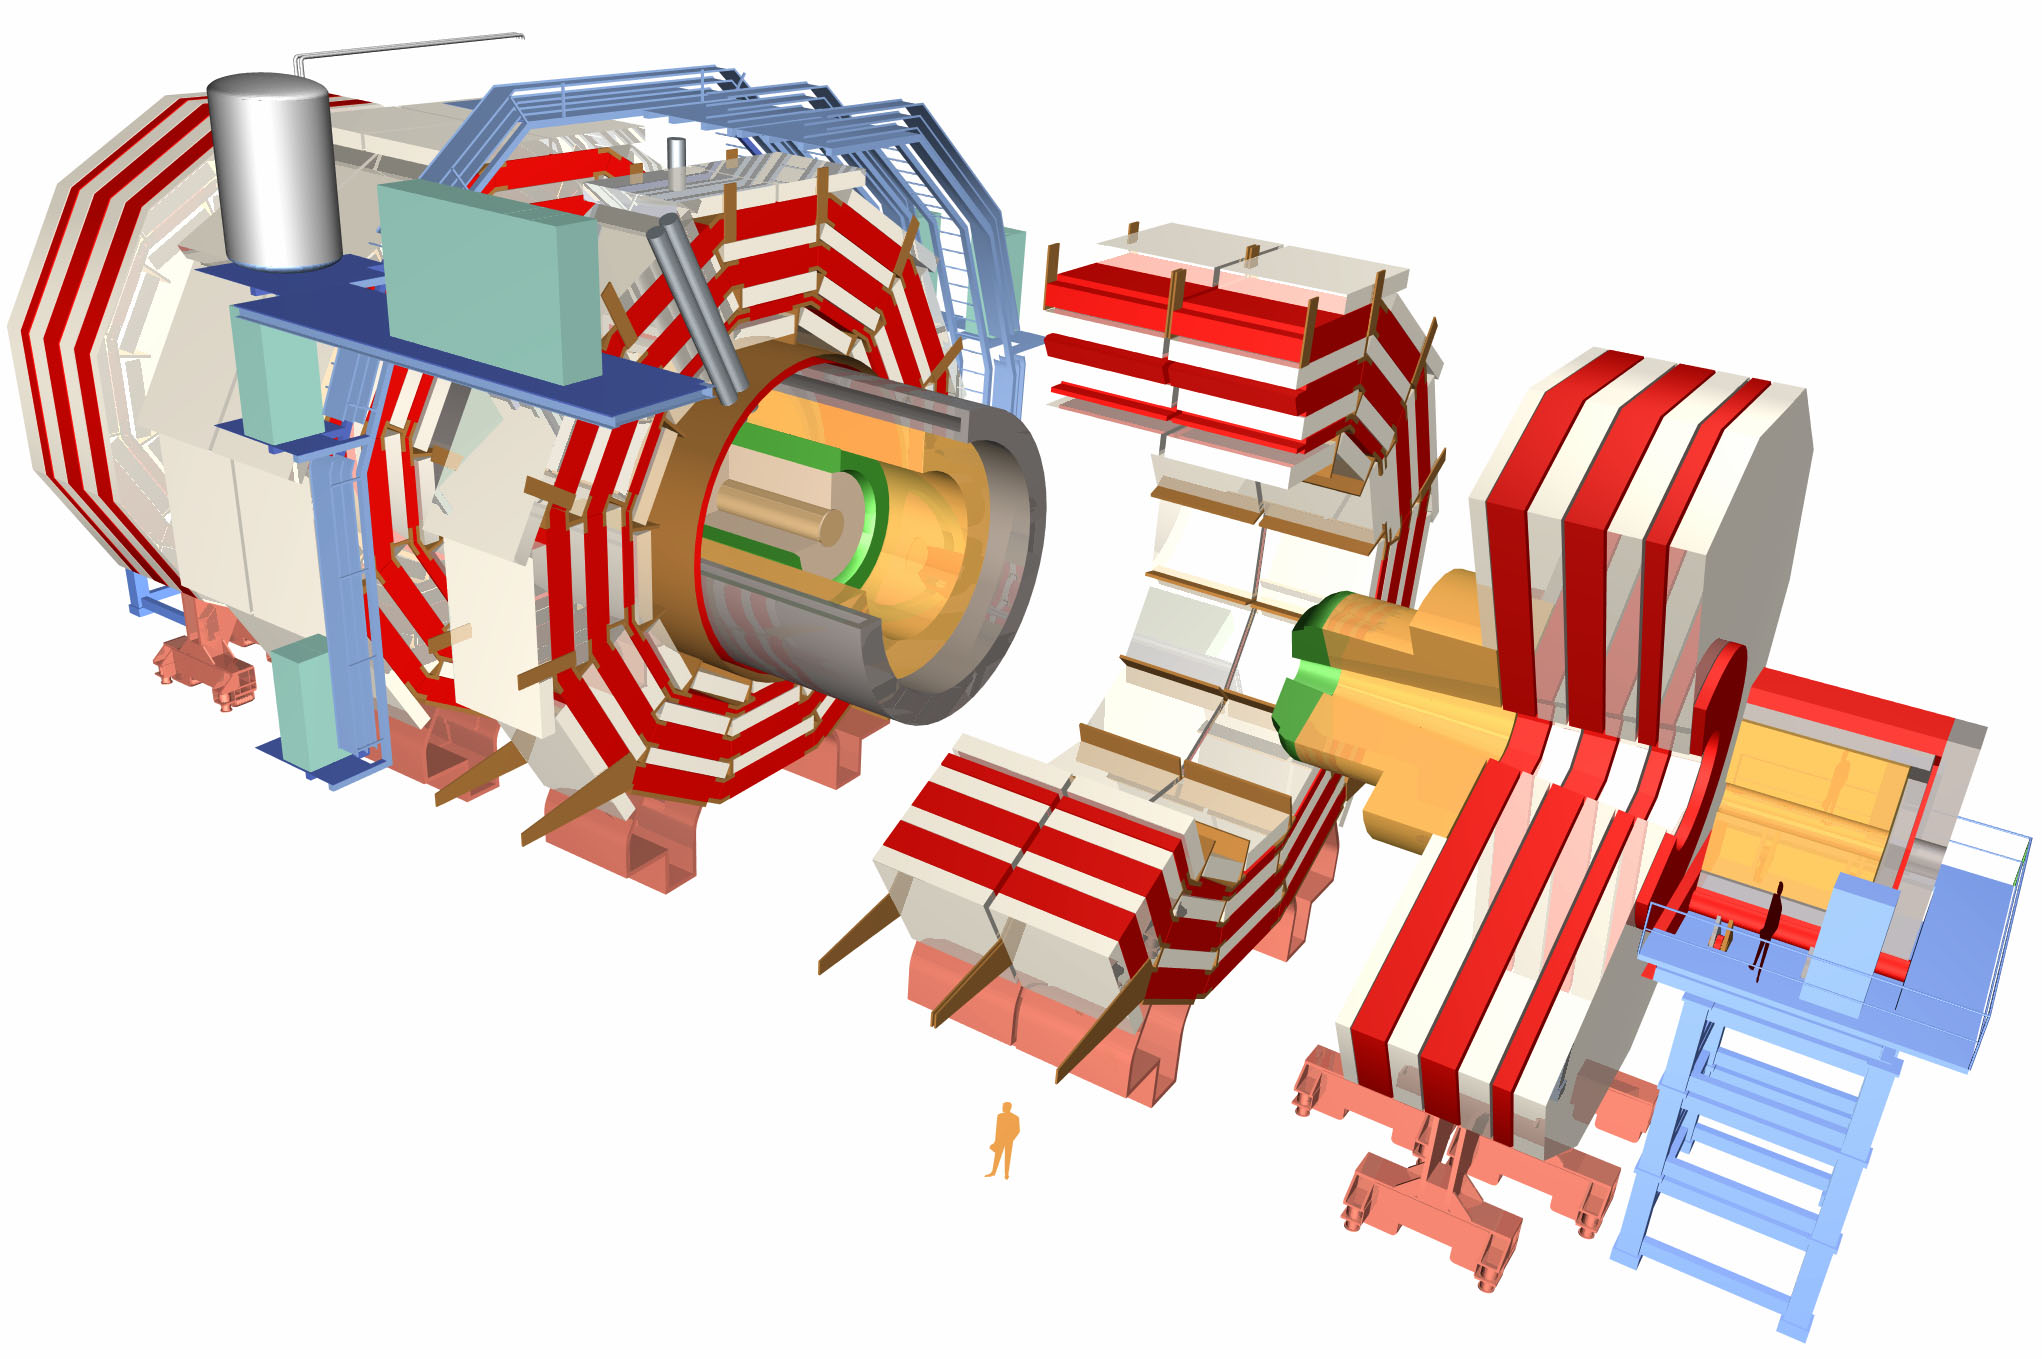
\includegraphics[width=0.95\textwidth]{lhc/CMSnc.jpg}
      }
    \end{column}
    \begin{column}{0.6\textwidth}
      \centering
      \only<3>{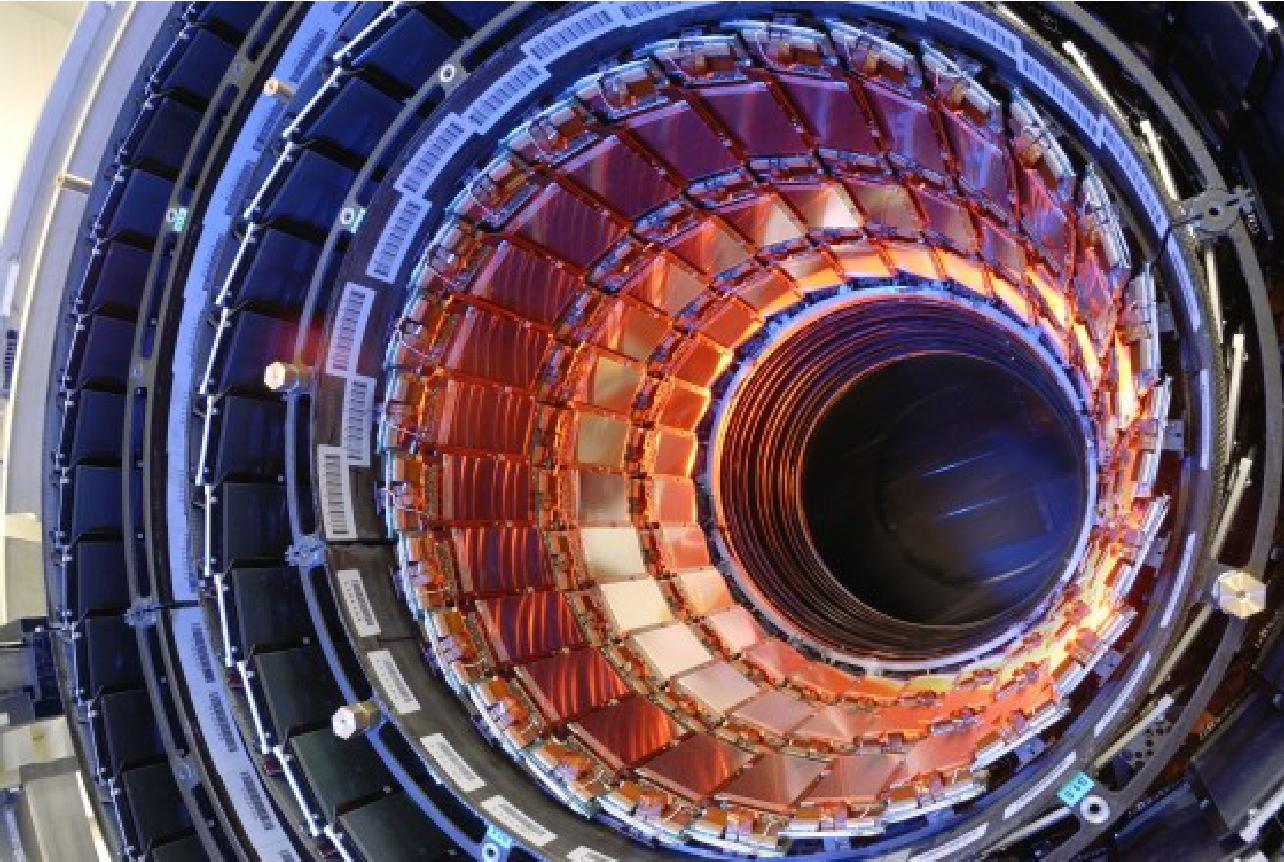
\includegraphics[width=0.95\textwidth]{lhc/Tracker.png}}
      \only<4>{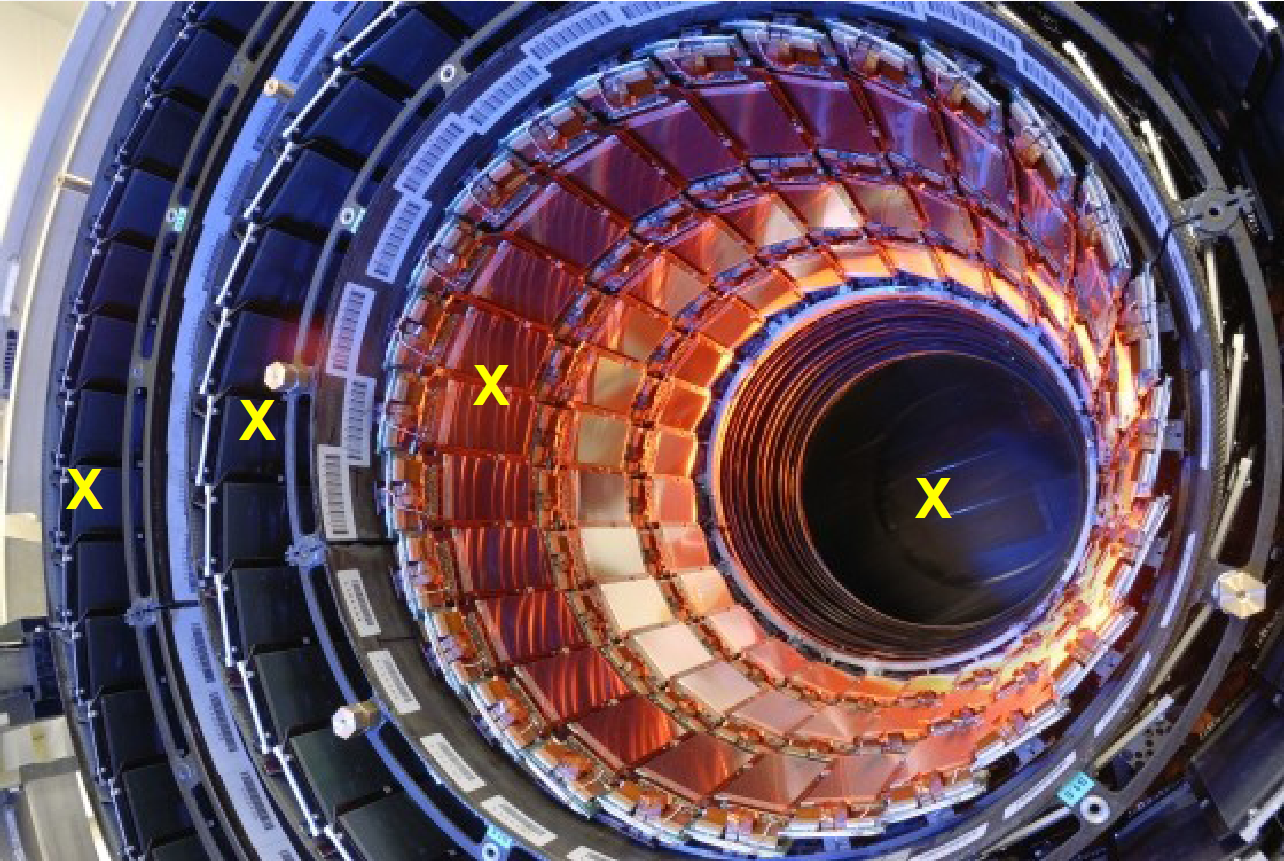
\includegraphics[width=0.95\textwidth]{lhc/Tracker_Hits.png}}
      \only<5->{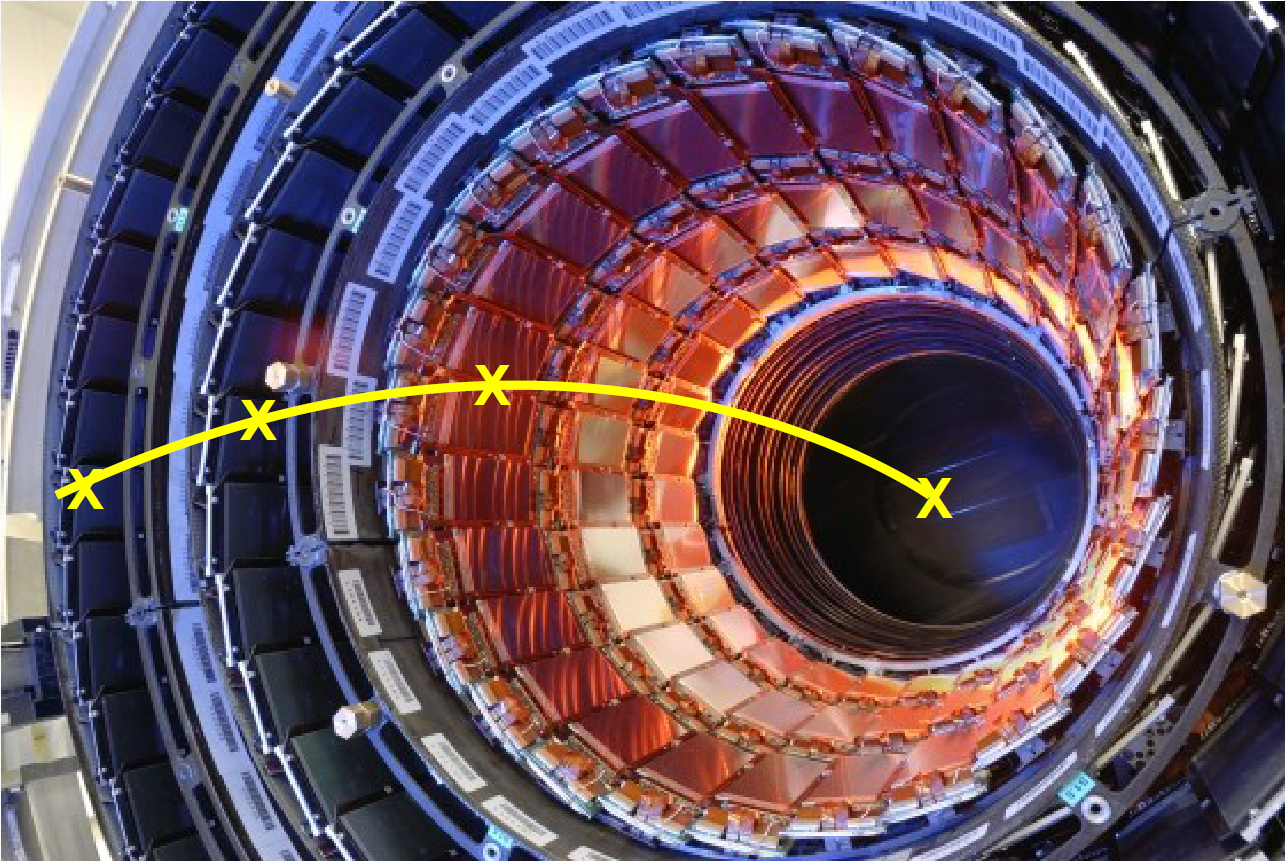
\includegraphics[width=0.95\textwidth]{lhc/Tracker_Hits_Track.png}}
    \end{column}    
  \end{columns}
\end{frame}

% --------------------------------------------------
\begin{frame}[t]
  \frametitle{Spurdetektor + Magnetfeld}
  \vskip0.3cm
  \begin{columns}
    \begin{column}{0.18\textwidth}
      \begin{block}{}
        \centering
        \textbf{Richtung}
      \end{block}
    \end{column}
    \begin{column}{0.025\textwidth}
    \end{column}
    \begin{column}{0.18\textwidth}
      \begin{block}{}
        \centering
        \textbf{Impuls}
      \end{block}
    \end{column}
    \begin{column}{0.025\textwidth}
    \end{column}
    \begin{column}{0.18\textwidth}
      \begin{block}{}
        \centering
        \textbf{Ladung}
      \end{block}
    \end{column}
    \begin{column}{0.025\textwidth}
    \end{column}
    \begin{column}{0.18\textwidth}
      \begin{block}{}
        \centering
        Energie
      \end{block}
    \end{column}
    \begin{column}{0.02\textwidth}
    \end{column}
    \begin{column}{0.18\textwidth}
      \begin{block}{}
        \centering
        \textcolor{white}{g}Teilchenart\textcolor{white}{g}
      \end{block}
    \end{column}
    \begin{column}{0.005\textwidth}
    \end{column}
  \end{columns}
  \vskip0.25cm
  \begin{columns}
    \begin{column}{0.4\textwidth}
      \centering
      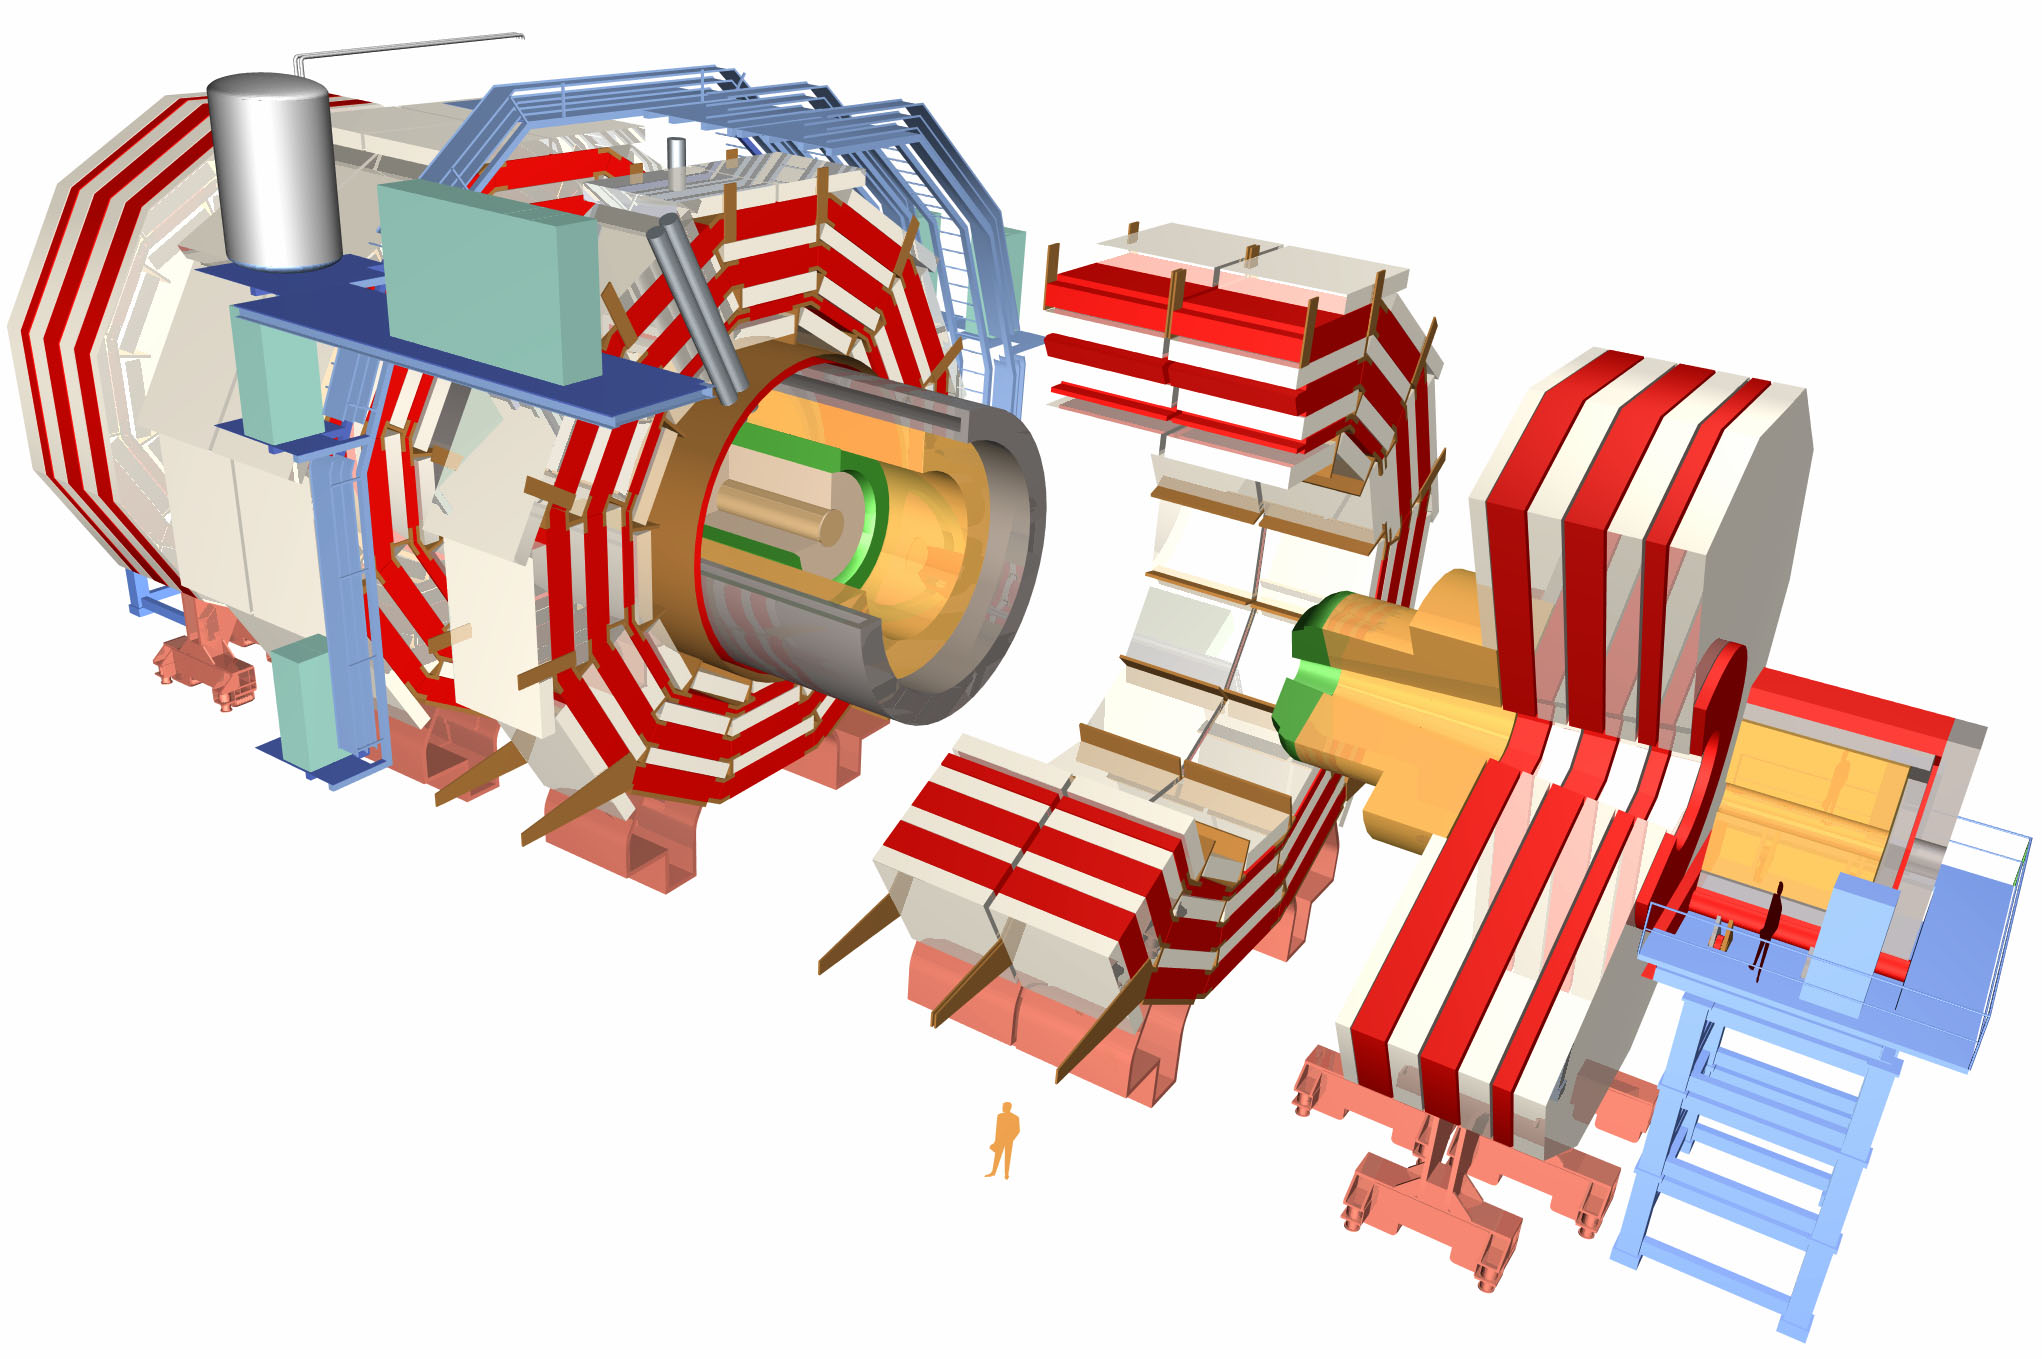
\includegraphics[width=0.95\textwidth]{lhc/CMSnc.jpg}
    \end{column}
    \begin{column}{0.6\textwidth}
      \centering
      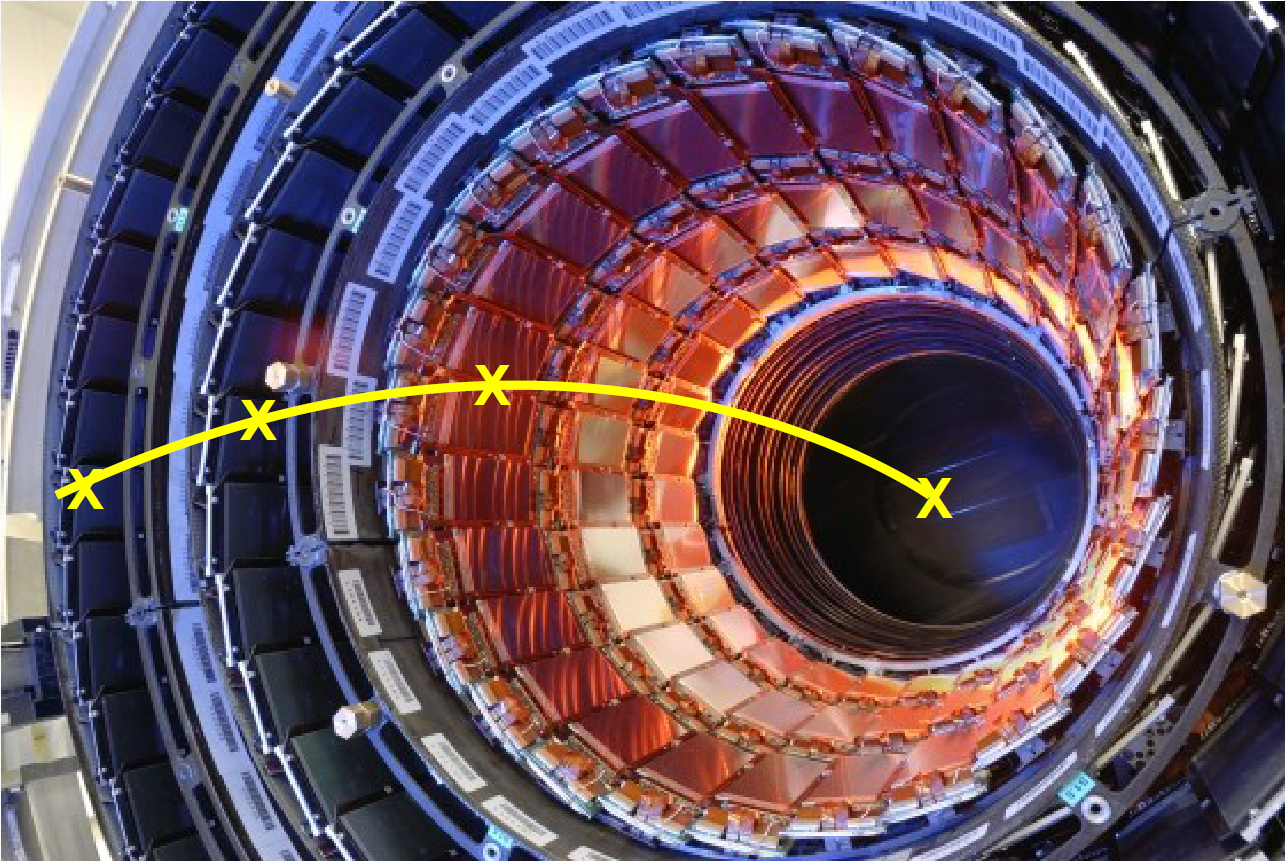
\includegraphics[width=0.95\textwidth]{lhc/Tracker_Hits_Track.png}
    \end{column}    
  \end{columns}
\end{frame}

% --------------------------------------------------
\begin{frame}[t]
  \vskip0.3cm
  \frametitle{Kalorimeter}
  \begin{columns}
    \begin{column}{0.18\textwidth}
      \begin{block}{}
        \centering
        \textbf{Richtung}
      \end{block}
    \end{column}
    \begin{column}{0.025\textwidth}
    \end{column}
    \begin{column}{0.18\textwidth}
      \begin{block}{}
        \centering
        Impuls        
      \end{block}
    \end{column}
    \begin{column}{0.025\textwidth}
    \end{column}
    \begin{column}{0.18\textwidth}
      \begin{block}{}
        \centering
        Ladung
      \end{block}
    \end{column}
    \begin{column}{0.025\textwidth}
    \end{column}
    \begin{column}{0.18\textwidth}
      \begin{block}{}
        \centering
        \textbf{Energie}
      \end{block}
    \end{column}
    \begin{column}{0.02\textwidth}
    \end{column}
    \begin{column}{0.18\textwidth}
      \begin{block}{}
        \centering
        \textcolor{white}{g}Teilchenart\textcolor{white}{g}
      \end{block}
    \end{column}
    \begin{column}{0.005\textwidth}
    \end{column}
  \end{columns}
  \vskip0.25cm
  \begin{columns}
    \begin{column}{0.4\textwidth}
      \centering
      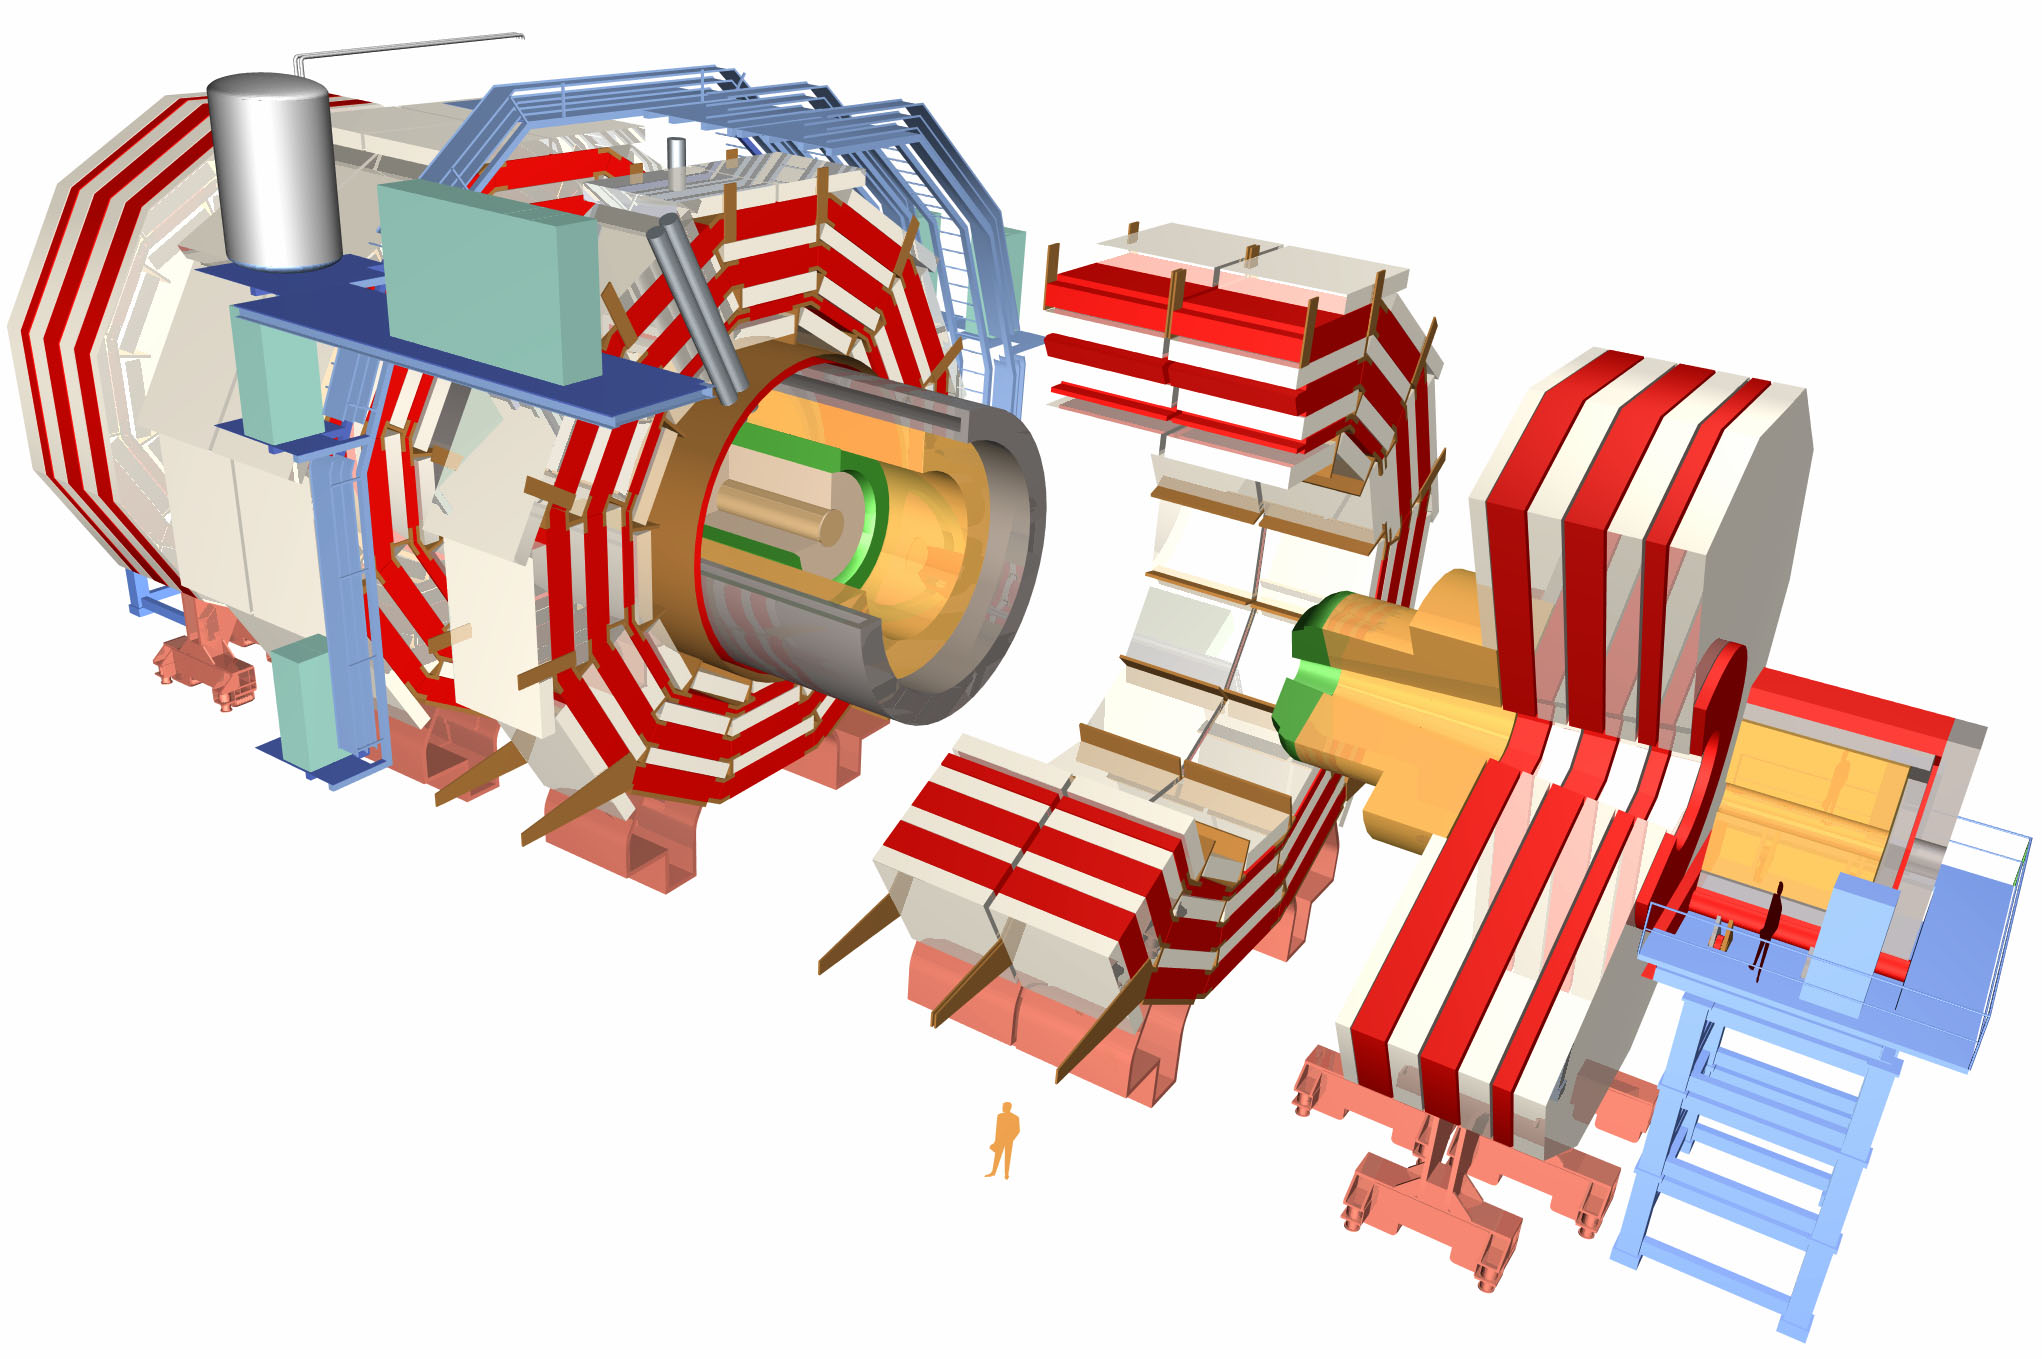
\includegraphics[width=0.95\textwidth]{lhc/CMSnc.jpg}
    \end{column}
    \begin{column}{0.6\textwidth}
      \centering
      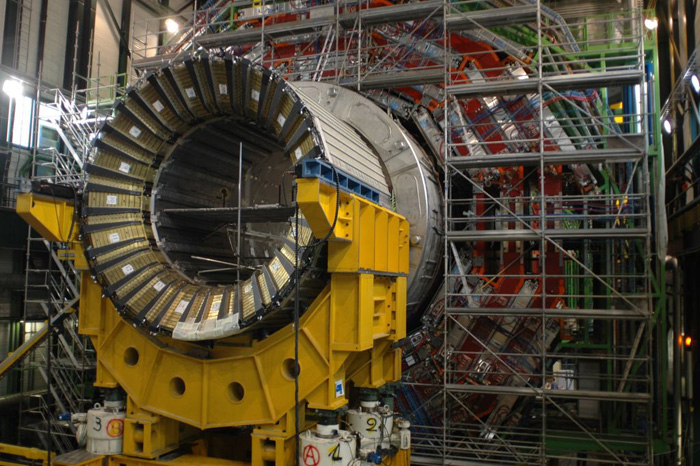
\includegraphics[width=0.95\textwidth]{lhc/CMS6.jpg}
    \end{column}    
  \end{columns}
\end{frame}

% --------------------------------------------------
\begin{frame}[t]
  \frametitle{Kombination aller Komponenten}
  \vskip0.3cm
  \begin{columns}
    \begin{column}{0.18\textwidth}
      \begin{block}{}
        \centering
        \textbf{Richtung}
      \end{block}
    \end{column}
    \begin{column}{0.025\textwidth}
    \end{column}
    \begin{column}{0.18\textwidth}
      \begin{block}{}
        \centering
        \textbf{Impuls}
      \end{block}
    \end{column}
    \begin{column}{0.025\textwidth}
    \end{column}
    \begin{column}{0.18\textwidth}
      \begin{block}{}
        \centering
        \textbf{Ladung}
      \end{block}
    \end{column}
    \begin{column}{0.025\textwidth}
    \end{column}
    \begin{column}{0.18\textwidth}
      \begin{block}{}
        \centering
        \textbf{Energie}
      \end{block}
    \end{column}
    \begin{column}{0.02\textwidth}
    \end{column}
    \begin{column}{0.18\textwidth}
      \begin{block}{}
        \centering
        \textcolor{white}{g}\textbf{Teilchenart}\textcolor{white}{g}
      \end{block}
    \end{column}
    \begin{column}{0.005\textwidth}
    \end{column}
  \end{columns}
  \vskip0.25cm
  \begin{center}
    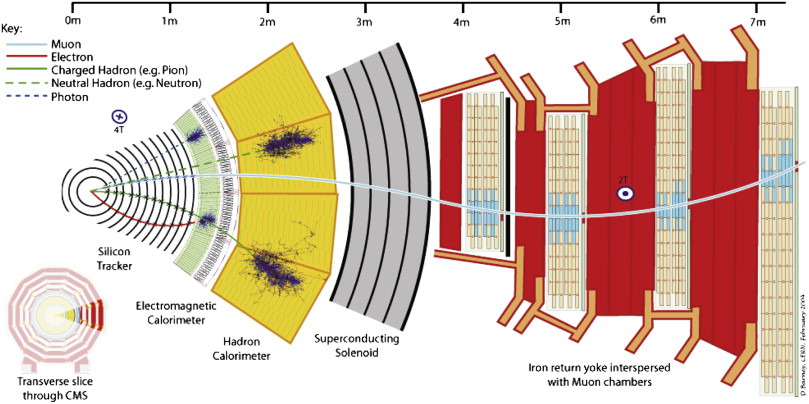
\includegraphics[width=\textwidth]{lhc/CMS-Wedge.jpg}
  \end{center}
\end{frame}

\section{Die LHC-Experimente}
% --------------------------------------------------
\begin{frame}
  \frametitle{Insgesamt vier gro\ss{}e Detektoren am LHC}
  \begin{block}{}
    \begin{description}[ATLAS]
    \item[CMS]<1-> Gibt es das Higgs? Gibt es noch weitere unbekannte Teilchen?
    \item[ATLAS]<2->  Gibt es das Higgs? Gibt es noch weitere unbekannte Teilchen?
    \item[LHCb]<3-> Warum gibt es mehr Materie als Antimaterie im Universum?
    \item[ALICE]<4-> Wie sah das Universum in den ersten Sekunden aus?
    \end{description}
  \end{block}
  \vskip0.2cm
  \begin{center}
    \only<1>{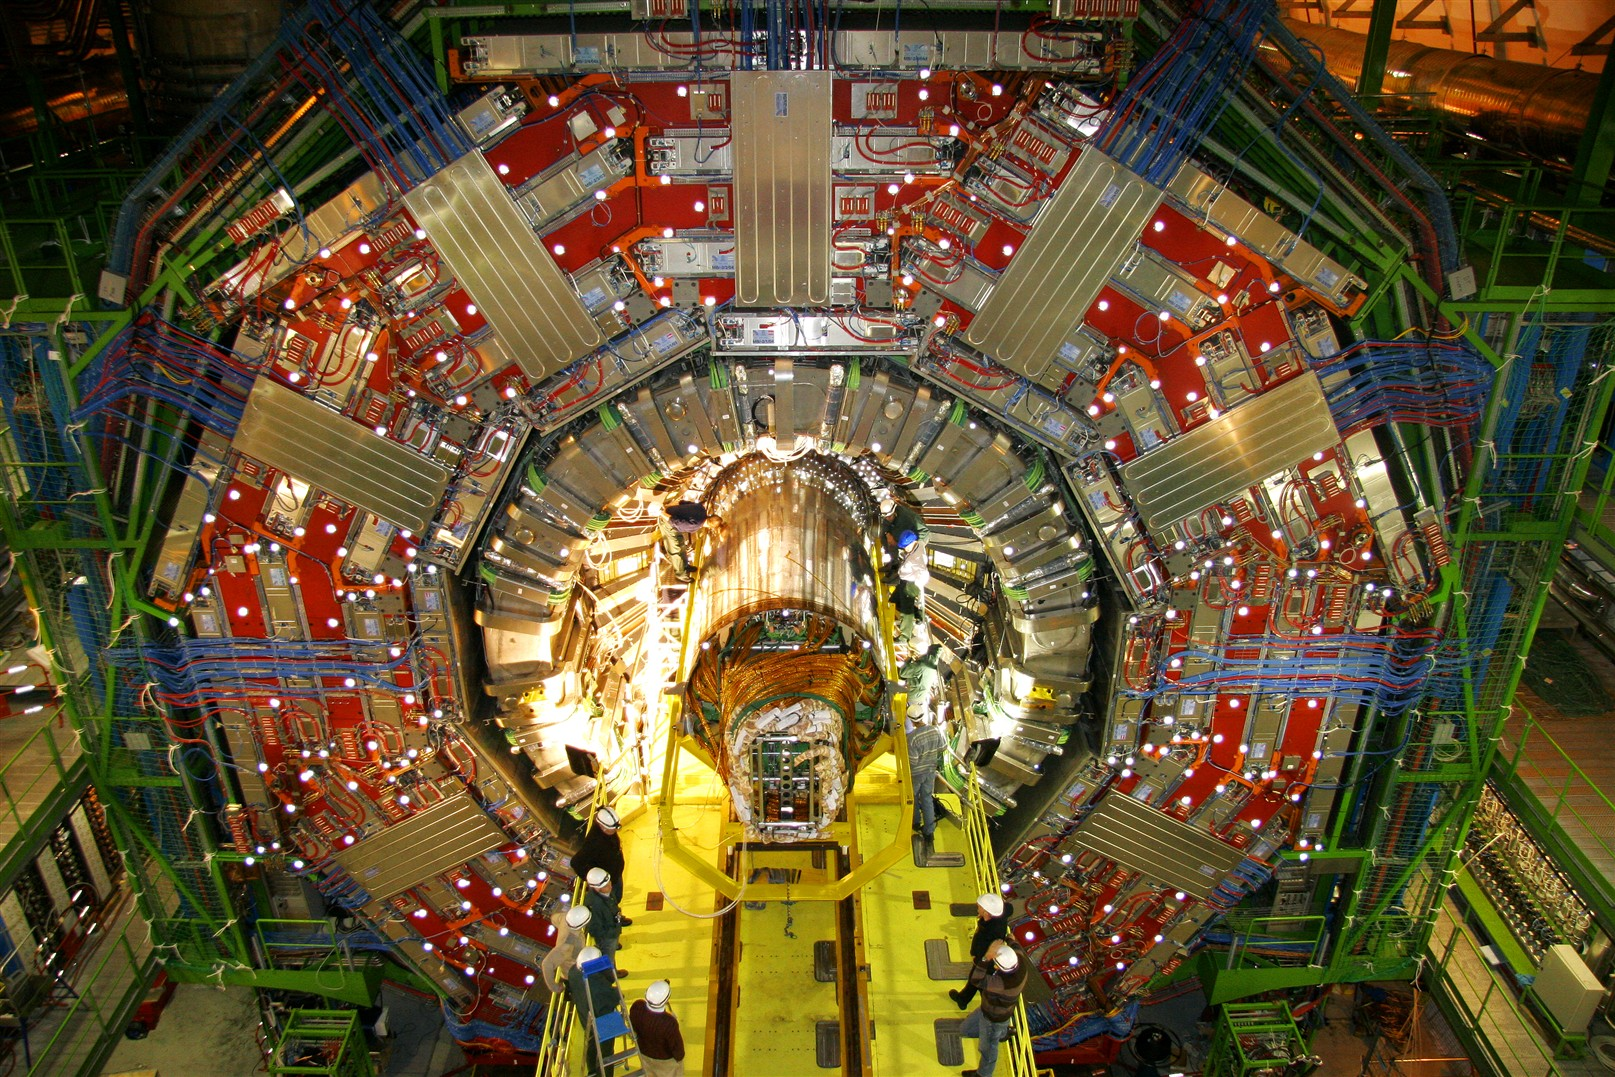
\includegraphics[height=0.5\textheight]{lhc/CMS_0712023_01-A4-at-144-dpi.jpg}}
    \only<2>{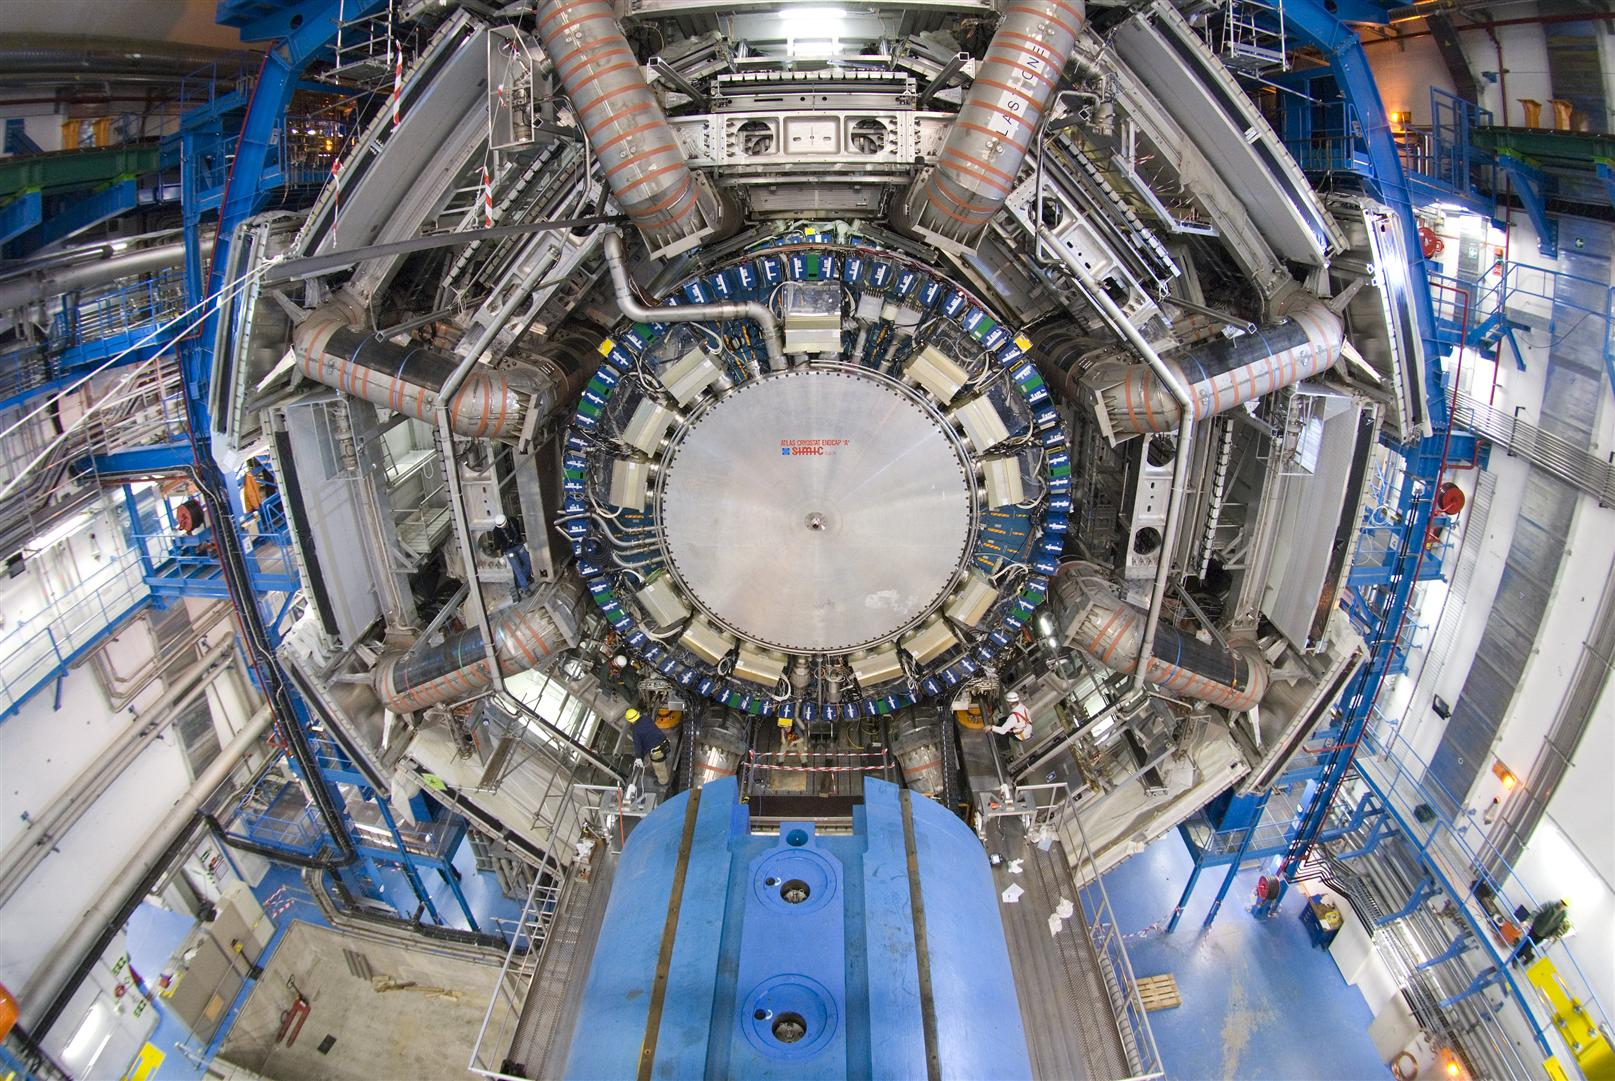
\includegraphics[height=0.5\textheight]{lhc/atlas2.jpg}}
    \only<3>{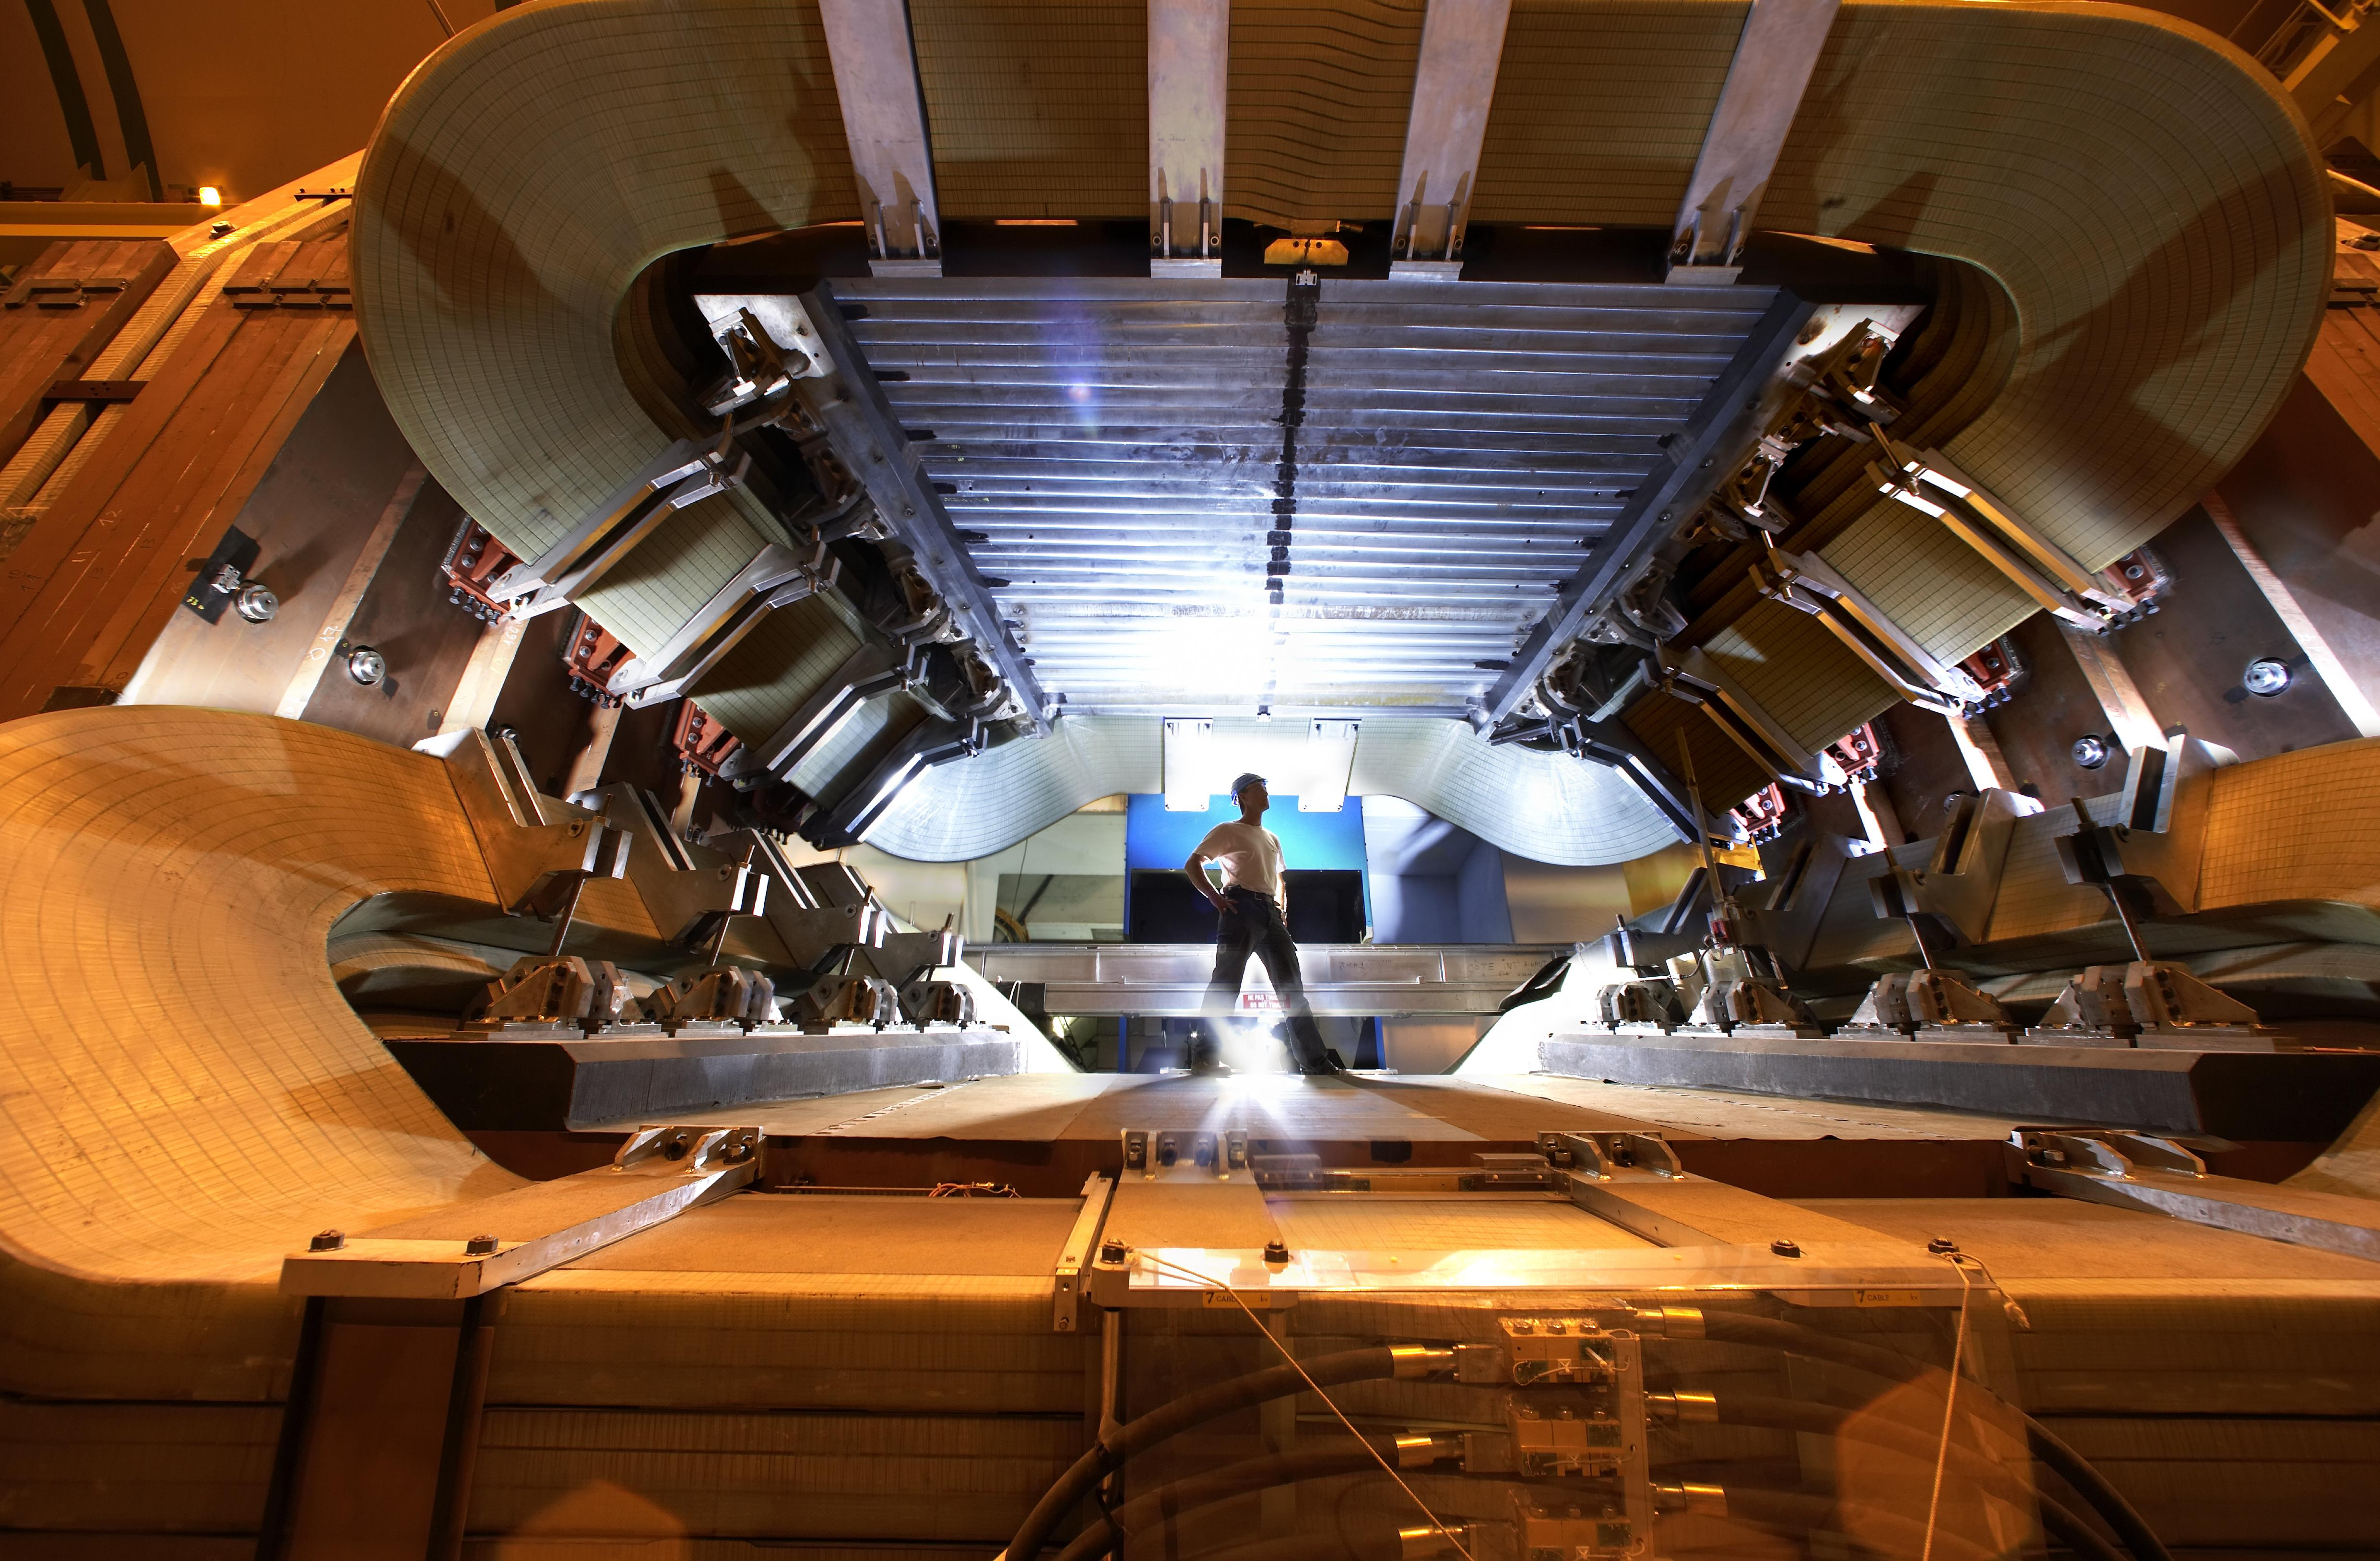
\includegraphics[height=0.5\textheight]{lhc/lhcb.jpg}}
    \only<4>{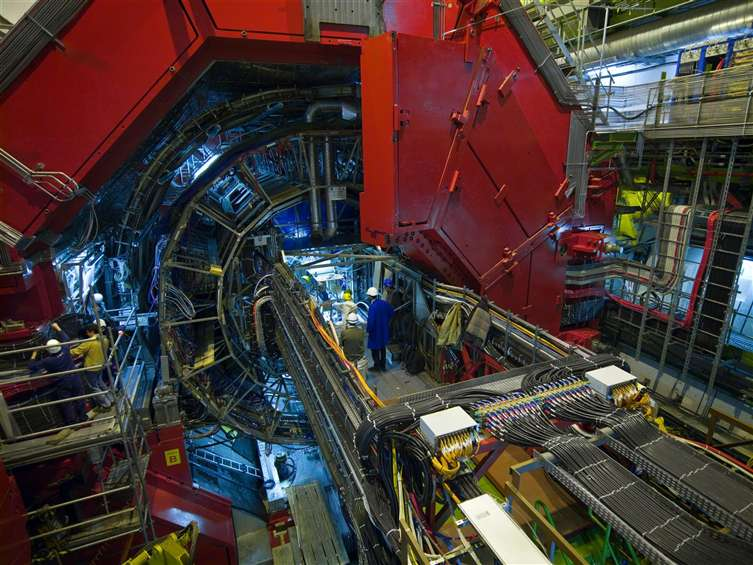
\includegraphics[height=0.5\textheight]{lhc/alice.jpg}}
  \end{center}
\end{frame}
